\documentclass{ieeeaccess}
\usepackage{cite}
\usepackage{amsmath,amssymb,amsfonts}
\usepackage{graphicx}
\usepackage{textcomp}
\usepackage{algorithm}
\usepackage[noend]{algpseudocode}%no closing statement
\usepackage[font=footnotesize]{caption}
\usepackage[font=footnotesize]{subcaption}
\usepackage{multicol}


\def\BibTeX{{\rm B\kern-.05em{\sc i\kern-.025em b}\kern-.08em
    T\kern-.1667em\lower.7ex\hbox{E}\kern-.125emX}}
\begin{document}
\history{Date of publication xxxx 00, 0000, date of current version xxxx 00, 0000.}
\doi{10.1109/ACCESS.2017.DOI}

\title{Interference minimization in D2D Communication Underlaying Cellular Networks}
\author{\uppercase{Md. Yeakub Hassan}\authorrefmark{1},
	\uppercase{Faisal Hussain\authorrefmark{1}, Md Sakhawat Hossen\authorrefmark{1}, Salimur Choudhury\authorrefmark{2} \IEEEmembership{Member, IEEE}, Muhammad Mahbub Alam\authorrefmark{1}\IEEEmembership{Member, IEEE}}}
\address[1]{Department of Computer Science and Engineering, Islamic University of Technology, Dhaka, Bangladesh (e-mail: yeakubhassan@iut-dhaka.edu, faisalhussain@iut-dhaka.edu, sakhawat@iut-dhaka.edu, mma@iut-dhaka.edu)}
\address[2]{Department of Computer Science, Lakehead University, Thunder Bay, Ontario, Canada (e-mail: salimur.choudhury@lakeheadu.ca)}

%\tfootnote{This paragraph of the first footnote will contain support 
%information, including sponsor and financial support acknowledgment. For 
%example, ``This work was supported in part by the U.S. Department of 
%Commerce under Grant BS123456.''}


%\author{\IEEEauthorblockN{Md Yeakub Hassan\IEEEauthorrefmark{1}, Faisal Hussain\IEEEauthorrefmark{1}, 
%  Md Sakhawat Hossen\IEEEauthorrefmark{1},
%Salimur Choudhury\IEEEauthorrefmark{2} and \\Muhammad Mahbub Alam\IEEEauthorrefmark{1}}
%
%\IEEEauthorblockA{\IEEEauthorrefmark{1}Department of Computer Science and Engineering, Islamic University of Technology, Dhaka, Bangladesh
%}
%
%\IEEEauthorblockA{\IEEEauthorrefmark{2}Department of Computer Science, Lakehead University, Thunder Bay, Ontario, Canada
%}
%Email:  \IEEEauthorrefmark{1}yeakubhassan@iut-dhaka.edu, 
% \IEEEauthorrefmark{1}faisalhussain@iut-dhaka.edu,
%\IEEEauthorrefmark{1}sakhawat@iut-dhaka.edu, \\\IEEEauthorrefmark{2}salimur.choudhury@lakeheadu.ca,  \IEEEauthorrefmark{1}mma@iut-dhaka.edu
%}


\markboth
{Hassan \headeretal: Interference minimization in D2D Communication Underlaying Cellular Networks}
{Hassan \headeretal: Interference minimization in D2D Communication Underlaying Cellular Networks}

\corresp{Corresponding author: Salimur Choudhury (e-mail: salimur.choudhury@lakeheadu.ca).}

\begin{abstract}
Interference minimization while maintaining a target system sum rate by sharing radio resources among cellular User Equipments (UEs) and Device-to-Device (D2D) pairs is an important research question in Long Term Evolution (LTE) and beyond (4G and 5G). Total system sum rate of a cellular network can be improved if cellular user equipments (UEs) and D2D pairs share resource blocks (RBs). However, some sharing can also decrease the sum rate and increase the system interference. Considering this observation, we address two types of assignments (Fair and Restricted) in resource allocation for the interference minimization resource allocation problem. We propose a two phase resource allocation algorithm for both fair and restricted assignments where our objective is to minimize the system interference and at the same time, maintaining a target system sum rate. In the phase-I of our proposed algorithm, a weighted bipartite matching algorithm is used to minimize the interference and get a feasible initial solution. In some cases, we can decrease the interference introduced in phase-I of our algorithm. Therefore, in the phase-II, local search techniques are used to improve the solution. We compare the fair assignment of our proposed algorithms with a two-phase auction based fair and interference aware resource allocation algorithm (TAFIRA) which addresses the same research problem. As well as, we compare the restricted assignment of our proposed algorithm with a Minimum Knapsack based Interference Resource Allocation algorithm (MIKIRA). We prove that MIKIRA fails to provide feasible solutions in most of the cases. We also show that the performance ratio of TAFIRA can be unbounded in the worst case. Moreover, in some cases, TAFIRA can not provide any solution to the problem though the solutions exist whereas our proposed algorithms always provide a solution whenever the solution exists. We perform extensive simulations of the algorithms and find that in all cases, our proposed algorithm outperforms a number of state-of-the-art algorithms.
\end{abstract}

\begin{keywords}
D2D, Interference Minimization, Sum rate, LTE, Hungarian, LP.
\end{keywords}


\titlepgskip=-15pt

\maketitle

\section{Introduction}
\label{sec:introduction}
\IEEEPARstart{I}{nterference} minimization is a mature research problem in the field of wireless and cellular communication. In recent days, a special attention is given to this area due to the introduction of a new mode of personal communication known as D2D communication underlay to a cellular network \cite{lte}. In this mode of communication, two near cellular UEs can communicate directly rather than communicating via eNB (Base Station in LTE). Different inter device applications and services like sharing documents in a conference, downloading media contents in a concert are some of the motivating examples where D2D communication can be a milestone rather than the conventional cellular communication \cite{doppler2009device}. Cooperative communications based on relaying node is very much promising in wireless networks for  power efficiency, spectral efficiency, and network coverage as well as capacity maximization. This is already been included in the fourth generation (4G) LTE advanced standard \cite{5g}. Next generation (5G) media-rich mobile applications require high data rates and capacity which is not possible in 4G networks. This demand for high data rates and capacity requires complicated reasoning for a 5G cellular system. D2D communication is recognized as one of the technology components of the emerging 5G architecture which can play a vital role in vehicle-to-vehicle communication and cellular network offloading. D2D communication increases bit-rate gain (as the distance between receiver and sender gets decreased), reuse gain (as both D2D devices and cellular UEs simultaneously use the common radio resources), hop-gain (as D2D communication uses a single link rather than using uplink and downlink resources for sending and receiving) and coverage gain (as D2D communication can be possible at some place where the signal strength of eNB is too low for cellular communication) \cite{fodor}. In addition, it consumes less power than communicating via eNB\cite{stefania}. Meanwhile, the spectral demand is also increasing day by day. Fortunately, D2D communication becomes convenient as LTE  introduces a provision to reuse the radio resources of a traditional cellular network. So allowing the reuse of licensed spectral band suffices the requirements. However, reusing radio resources can introduce potential interference in the network. Although LTE uses  Orthogonal Frequency Division Multiplexing (OFDM) technique to avoid interference, due to a bad design, sharing resources with D2D devices may introduce potential co-channel interference in the cellular network which can affect the primary users \cite{asadi2014survey, min}. 

\smallskip
\noindent
Several research works are ongoing where researchers are deploying different aspects like maximizing sum rate, minimizing interference, management of transmission power etc \cite{lora}, \cite{zulhasnine}, \cite{islam2016radio}. Network providers may want to minimize the interference to prioritize the primary users while accommodating the D2D communication by sharing resources to achieve a certain system sum rate \cite{islam2016radio, islam2015reducing}. An efficient resource allocation technique can assign suitable resource blocks (RBs) to the D2D pairs to avoid the above mentioned problem. Most of the existing algorithms consider that sharing can only improve the system sum rate. However, some of the sharing (assignments) can also decrease the system sum rate \cite{ccnc}. This paper focuses on this problem area and proposes a resource allocation algorithm which minimizes the system interference due to resource sharing and at the same time maintains a target system sum rate. 

\smallskip
 
The key contributions of this paper is, we consider two types of assignment schemes for resource allocation, one of them is fair assignment scheme where all D2D pairs have the flexibility to share RBs of any cellular UEs and another one is restricted assignment scheme where D2D pairs are blocked to share RBs of any cellular UEs if their sharing decreases the system sum rate. As well as, we propose a two phase interference minimization resource allocation algorithm for both types of assignment scheme. In the phase-I of the proposed algorithm, a weighted bipartite matching approach is used to solve the interference minimization problem and in the phase-II, local search techniques are used to improve the solution of phase-I. Network providers can use any of the proposed assignment schemes in our resource allocation algorithm. Our proposed algorithm always guarantees a solution whenever it exists, while existing algorithms do not guarantee this. Simulation results show that our proposed resource allocation algorithm provides better performances than a number of state-of-the-art algorithms. The initial version of this paper (restricted assignment) can be found in \cite{icc}.
 
\smallskip
 
The rest of the paper is designed in the following manners. Section \ref{sec:relatedworks} canvasses prior works related to our topic of interest. Section \ref{sec:systemModel} and \ref{sec:problemFormulation} contains the system and channel model of our problem and the problem formulation respectively. Section \ref{existingAlgorithms} discusses existing resource allocation algorithms for our research problem and their flaws. Section \ref{section:algorithm} presents a detailed discussion of our proposed algorithm with working procedures. The performance evaluations are  shown in section \ref{section:FairPerformance}. Finally, section \ref{sec:conclusion} draws the conclusion.

\section{Related Works}\label{sec:relatedworks}
 
Numerous research works have been conducted on various resource allocation problems of D2D communication underlaying cellular networks. In literature we can find several studies reviewing different scope of research e.g. resource allocation, power control, admission control, massive multiple-input-multiple-output, time scheduling, network coding, designing protocol etc. for D2D communication \cite{mach2015band,asadi2014survey}. This paper focuses on the area of interference minimization of a system while maintaining a target system sum rate where D2D communication takes place underlaying LTE cellular networks. There are two existing algorithms (TAFIRA and MIKIRA) that consider the same problem we are considering. A knapsack based interference aware resource allocation named as MIKIRA is proposed in \cite{islam2015reducing}. The goal of MIKIRA is to minimize the total interference as well as  maintain a system sum rate demand. They use a knapsack based approximation algorithm to solve the resource allocation problem. MIKIRA stops allocating RBs to D2D pairs as soon as the demand of target sum rate is met. Therefore, the algorithm is not fair in terms of resource allocation as some D2D pair may not get any cellular UE's resources. However, in most of the cases, the algorithm does not give the feasible solution where some D2D pairs use multiple cellular UE's resources as well as some cellular UEs share their resources with multiple D2D pairs which contradict the formulation of their optimization problem. 

\smallskip
 
TAFIRA, a two phase auction based fair resource allocation algorithm is proposed in \cite{islam2016radio} that also consider the problem where the objective is to minimize the system interference by maintaining a target system sum rate. However, it allocates each D2D pair to at least one cellular UEs using a greedy choice and then, tries to minimize the total system interference. TAFIRA has two phases where the first phase aims to assign resources in such a way that it incurs minimum interference while assigning every D2D pair to a cellular UE in the system and in the second phase a local search algorithm tries to increase the sum rate by swapping the allocated RBs with the unallocated cellular UEs. TAFIRA also suffers from infeasible solutions. Moreover, in the worst case, the performance ratio of TAFIRA is unbounded. 

\smallskip
 
Zhang  \textit{et al.} \cite{rzhang} present an interference aware graph based resource allocation for downlink scenario.  However, they do not provide any result in the improvement of signal quality. In \cite{xu}, an auction based approach is proposed where the total resource is divided into homogeneous units and the value of a unit is calculated from channel capacity gain. An analysis of D2D communication on both spectrum overlay and underlay of an existing cellular network with ad hoc networks is discussed in \cite{huang}. They apply a technique called Successive Interference Cancellation (SIC), which generates good transmission capacity. Peng \textit{et al.} \cite{peng2009interference} propose interference tracing approach to mitigate the interference from the cellular transmission to the D2D communication and use tolerable interference broadcasting approach to mitigate the interference generated other way around. Multiple Input Multiple Output (MIMO) transmission scheme in cellular downlink is proposed in \cite{janis2009interference} to avoid elaborated interference to D2D communication. Yin \textit{et al.} \cite{yin2013distributed} formulate the resource allocation problem into the Stackleberg game problem to derive distributed scheme. Interference Suppression Area (ISA) is introduced to manage the interference at cell edge in \cite{guo2014interference}. Interference limited area for cellular UEs has been suggested in \cite{min2011capacity} where D2D devices can share the uplink medium. On the other hand, a restricted zone is modeled in downlink medium in \cite{cai_cap}. Both of the works find a candidate set of D2D devices for allocation. However, the allocation of candidate D2D devices is not guaranteed to be optimal. In \cite{du}, an interference controlled D2D routing design is proposed where multi-hop D2D transmission upgrades flexibility of future cyber-physical systems (CPSs). However, these works are not same as our settings rather similar to our problem.

\smallskip
 
Several research works have been done in the area of sum rate maximization of a system where D2D communication takes place underlay to a cellular network. A bipartite matching approach in \cite{jiang}, is proposed to solve resource allocation problem for maximizing the system sum rate for downlink and uplink scenario. They use the Kuhn-Munkres (KM) algorithm to solve the bipartite matching problem. However, they do not consider system interference in the problem formulation. They overlook the situation where sharing RBs can decrease the system sum rate. A simple local search algorithm is designed in \cite{lora} to solve the same resource allocation problem (maximizing system sum rate while maintaining some QoS). A deferred acceptance based resource allocation algorithm (DARA) is proposed in \cite{dara} to solve the same problem following a stable matching algorithm. Nevertheless, these works are not directly related to our research problem.

\smallskip
 
Several emerging research works, that have been done in D2D communication field, are discussed in the following. Zhang et al. \cite{zhang2017interference} propose a two-stage interference graph construction protocol for D2D communication underlaid a cellular network where the first stage is used to announce the existence of a D2D link to its neighbor area and the second stage of the protocol is dealing with the collision resolution that could occur in the announcement stage. Both of the stages work in an iterative manner where the interference graph construction is considered as link-level neighbor discovery procedure rather than the conventional device-level neighbor discovery procedure.


\smallskip
 
Wang et al. \cite{wang2017power} revisit the problem of power control for multiple interfering D2D communication and propose an approximate interior point method to maximize the sum rate of the D2D pairs underlaying cellular network. To develop a low complexity solution they investigate the properties of the Hessian matrix in power control problem and replace the time consuming inversion of Hessian matrix with its diagonal which results in lower computation complexity.
 


\smallskip
 
Ding et al. \cite{ding2016cellular} focus on the exploration of unlicensed TV white spaces (TVWS) for D2D communication by exploiting the existing cellular infrastructure. They propose a systematic approach to build a geo-location database with a lookup table service for a D2D link to determine its maximum permitted emission power (MPEP) in the unlicensed digital TV band. To achieve this they formulate an optimization problem of maximizing the re-usability of a TV channel between licensed digital TV service and unlicensed D2D communication and introduce the concept of crowd sensing to collect active spectrum measurement from the huge number of user hand held devices. They propose an opportunistic spatial reuse algorithm  to determine the MPEP of a D2D link and develop big spectrum data mining algorithms to implement the geo-location database service.


\smallskip
 
There are some other very recent research works on D2D communication targeted for 5G which is evolving from system-centric  to user-centric system \cite{marsch2016preliminary,chen2016user} focusing on different performance metrics for various network edge services. Although the research problem we are addressing is not directly related to these works, we find them very interesting and would like to mention some of the notable works \cite{tang2017user,tangcapacity}. In \cite{tang2017user} an user-centric admission control method coupled with resource allocation technique is proposed for 5G D2D extreme mobile broadband. The proposed method applies the sequential convex programming technique to get a reasonable approximation of the optimal solution. Tang et al. \cite{tangcapacity} proposes a two-step capacity oriented resource allocation technique for D2D communication underlaying cellular network. In step one they propose a joint admission control and resource allocation scheme for the maximization of system capacity while maintaining the individual QoS requirements of the primary users using graph based solution. In step two they control the power of the admitted D2D devices to enhance the system-wide parameters like energy conservation, system throughput, energy efficiency, minimum individual data rates etc.


\section{System Model and Channel Model}\label{sec:systemModel}
 
We consider the same system model and channel model used in \cite{islam2016radio}, \cite{islam2015reducing}, \cite{islam2015reducing_old}. We consider that D2D communication is undergoing using the uplink radio resources of LTE cellular network. While reusing the uplink resources, D2D receivers encounter interference from cellular UEs. On the other hand, eNB faces interference from the D2D transmitters \cite{islam2016radio}. It is noted that in such an underlay system D2D pairs can communicate with each other directly but eNB \cite{zulhasnine} handles the connection establishment and the resource allocation. Here, we consider a system with one eNB, $n$ cellular UEs and $m$ D2D pairs ($n>>m$) where the set of cellular UEs is represented as $C = \{c_{1}, c_{2}, c_{3}, ..., c_{n}\} $ and the set of D2D pairs is represented as $D = \{ d_{1}, d_{2}, d_{3}, ..., d_{m} \}$. In the rest of the paper, cellular UEs are denoted as $c_i$ for each $1$ $\leq$ $i$ $\leq$ $n$ and D2D pairs are denoted as $d_j$ for each $1$ $\leq$ $j$ $\leq$ $m$. Each D2D pair $d_j$ consists of a transmitting device $d_j^t$ and a receiving device $d_j^r$. We assume our system as an Urban Micro System which follows Rayleigh fading path loss model \cite{islam2016radio,zulhasnine} where channels are considered to be orthogonal and each cellular UE uses separate RBs. Thus inter channel interference is absent but co-channel interference may present if any D2D pair is reusing the channel. The path loss (dB unit) model in the proposed system is \cite{zulhasnine} 
\begin{equation}
PL = 36.7\log_{10}(dist)+22.7+26\log_{10}(f_{c}),
\end{equation}
where $dist$ (meter) is the distance between D2D transmitter and receiver and $f_{c}$ (GHz) is the frequency of communication medium. The value of  $f_{c}$ is mentioned in the table~\ref{Simulation_table}.
The channel gain between these two devices is \cite{zulhasnine} 
\begin{equation}
G^{a,b} = 10^{-PL^{a,b}/10},
\end{equation}
where $a$ and $b$ are the sending and receiving devices respectively. $PL^{a,b}$ is the distance dependent path loss between $a$ and $b$. 

\section{Problem Formulation}\label{sec:problemFormulation}
\smallskip
  
This paper deals with an assignment problem, where each D2D pair $d_j$ is assigned to a cellular UE $c_i$ in the system. An assignment implies that a D2D pair is sharing the RBs of its assigned cellular UE. Our goal is to find a set of assignments which incur minimum interference due to resource sharing while maintaining a target system sum rate.
  
\smallskip

In the followings, a number of equations are stated which are necessary for the addressed research problem. Assume that the transmission power of a cellular UE $c_i$, D2D transmitter $d_j^t$ and eNB are $P^{c_i}$, $P^{d_j^t}$ and $P^{eNB}$ respectively. We also consider $\sigma$ as the thermal noise at the receiver end, also known as the energy of Additive White Gaussian Noise (AWGN). It is noted that maximum one D2D pair can reuse the RBs of a cellular UE. Signal to Interference plus Noise Ratio (SINR) at the eNB in uplink phase while communicating with a cellular UE $c_i$ (provided that D2D pair $d_j$ is reusing the same RBs) is 
\begin{equation}\label{eqn:sinr_enb}
\gamma_{c_i,d_j} = \frac{P^{c_i}G^{c_i,eNB}}{\sigma + P^{d_{j}^{t}}G^{d_{j}^{t},eNB}},
\end{equation}

where $G^{d_{j}^{t},eNB}$ implies channel gain between the D2D transmitter $d_{j}^t$ and the eNB, and $G^{c_i,eNB}$ implies the channel gain between the eNB and the cellular UE $c_i$ \cite{islam2015reducing}. If no D2D pair reuses the RBs of $c_i$, the equation~(\ref{eqn:sinr_enb}) can be rewritten as  

\begin{equation}\label{eqn:sinr_enb0}
\gamma_{c_i,0} = \frac{P^{c_i}G^{c_i,eNB}}{\sigma},
\end{equation}

 
where the co-channel interference is zero because no D2D pair is sharing the RBs of the cellular UE $c_i$. Similarly, the SINR at D2D receiver reusing uplink resources (provided that the D2D pair $d_j$ is reusing the same RBs of $c_i$) is
\begin{equation}\label{eqn:sinr_d}
\gamma_{d_j,c_i} = \frac{P^{d_{j}^t}G^{d_{j}^t,d_{j}^r}}{\sigma + P^{c_i}G^{c_i,d_{j}^r}},
\end{equation}

where $G^{d_{j}^t,d_{j}^r}$ denotes the channel gain between the D2D transmitter $d_{j}^t$ and the D2D receiver $d_{j}^r$.
Hence the total interference is originated in the system due to sharing of resources by cellular UE $c_i$ and D2D pair $d_j$ is
\begin{equation}\label{eqn:interference}
I_{c_i,d_j} = P^{d_j^t}G^{d_{j}^t,eNB} + P^{c_i}G^{c_i,d_{j}^r}.
\end{equation}


According to Shannon's capacity formula \cite{forouzan}, sum rate contribution of a cellular UE $c_i$ (provided that D2D pair $d_j$ is sharing the resources) can be represented as 
\begin{equation}\label{eqn:sumrate}
S_{c_i,d_j} = B\log_{2}(1+\gamma_{c_i,d_j}) + B\log_{2}(1+\gamma_{d_j,c_i}),
\end{equation}

where $\gamma_{c_i,d_j}$ indicates the SINR at eNB while communicating with cellular UE $c_i$ and $\gamma_{d_j,c_i}$ indicates the SINR at D2D receiver $d_{j}^r$ while communicating with D2D transmitter $d_{j}^t$ and $B$ is the bandwidth of the channel. If no D2D pair reuses the RBs of cellular UE $c_i$, then  the sum rate contribution of cellular UE $c_i$ is
\begin{equation}\label{eqn:sumrate_0}
S_{c_i,0} = B\log_{2}(1+\gamma_{c_i,0}).
\end{equation}

So, the total system sum rate $Z$ can be expressed as 
\begin{equation}\label{eqn:sumrate_total}
Z=\sum_{i = 1}^{n}(1 - \sum_{j = 1}^{m} x_{i,j}) S_{c_i,0}N_{c_i}+\sum_{i = 1}^{n}\sum_{j = 1}^{m} x_{i,j} S_{c_i,d_j} N_{c_i},
\end{equation}

where $N_{c_i}$ implies the number of RBs allocated to a cellular UE $c_i$ and $x_{i,j}$ is a binary variable that indicates whether a D2D pair $d_j$ shares the RBs of a cellular UE $c_i$ or not. It is noteworthy that, RA algorithm sets the value of $x_{i,j}$ and its range is fixed by the constraint (\ref{eqn:constraintx}).  The first part of this equation calculates the total sum rate contribution of the unassigned cellular UEs where $S_{c_i,0}$ represents the sum rate contribution of an unassigned cellular UE $c_i$. The second part of this equation calculates the total sum rate contribution of the assigned cellular UEs with the D2D pairs where $S_{c_i,d_j}$ represents the sum rate contribution of a cellular UE $c_i$ and a D2D pair $d_j$ when $d_j$ reuses the RBs of $c_i$. If we assume $T$ as the target system sum rate, then the objective function can be formulated as

\begin{align}
&\text{minimize} \sum_{i=1}^{n}\sum_{j=1}^{m} x_{i,j} I_{c_i,d_j}  \label{eqn:objective} \\
\text{sub}&\text{ject}\text{ to,}\notag\\
&Z \geqslant T \label{eqn:constrain_target}\\
&\sum_{j=1}^{m}x_{i,j} \leqslant 1\;; \quad \forall \;c_i \in C \;\;\;\;\;\;\;\;\;\;\;\;\;\;\;\;\;\;\;\;\;\;\;\;\;\;\;\;\;\;  \label{eqn:constraintxc}
\end{align}
\begin{subequations}
\begin{align} 
&\sum_{i=1}^{n}x_{i,j} = 1\;; \quad \forall \;d_j \in D \;\;\;\;\;\;\;\;\;\;\;\;\;\;\;\;\;\;\;\;\;\;\;\; \label{eqn:constraintFair}\\
&\sum_{i=1}^{n}x_{i,j} \leqslant 1\;; \quad \forall \;d_j \in D \label{eqn:constraintRestricted}
\end{align} 
\end{subequations}
\begin{align} 
&x_{i,j} \in \{0,1\}\;; \quad \forall \;c_i \in C \;  \text{and} \; \forall \;d_j \in D \;\; \label{eqn:constraintx}
\end{align} 

\smallskip

Sharing RBs of a single cellular UE with more than one D2D pair generates higher interference and sharing RBs of different cellular UEs by a single D2D pair makes the system complex. So in our proposed system, multiple sharing is avoided. Constraint~(\ref{eqn:constraintxc}) implies that a cellular UE can share RBs with the maximum of one D2D pair. 
Constraint~(\ref{eqn:constraintFair}) implies that a D2D pair must share RBs with only one cellular UE and constraint~(\ref{eqn:constraintRestricted}) implies that, a D2D pair can share RBs with maximum one cellular UE or it can remain unassigned. Depending on these constraints, we present two types of assignment scheme to minimize the objective function~(\ref{eqn:objective}). We define \textbf{Fair Assignment Resource Allocation (FARA)} scheme where each D2D pair of the system must share RBs of exactly one cellular UE. It ensures the ``fairness" property (same as TAFIRA) of the interference minimization resource allocation problem. Constraint~ (\ref{eqn:constraintFair}) is used to define the fair assignment property of this resource allocation problem. 

\smallskip
 
In some cases, sharing RBs between a D2D pair and a cellular UE can also decrease the system sum rate \cite{ccnc, cai_cap}. Considering this, we define \textbf{Restricted Assignment Resource Allocation (RARA)} scheme where a cellular UE $c_i$ does not share RBs with a D2D pair $d_j$, if $S_{c_i,d_j} < S_{c_i,0}$, which concludes that either a D2D pair shares RBs of the maximum of one cellular UE or it remains unassigned with any of the cellular UEs. In this case, we replace constraint (\ref{eqn:constraintFair}) by constraint (\ref{eqn:constraintRestricted}) to define the restricted assignment property of this resource allocation problem. It is noted that, though TAFIRA \cite{islam2016radio} and MIKIRA \cite{islam2015reducing} both consider constraint (\ref{eqn:constraintRestricted}) in their problem formulations, MIKIRA does not follow the fairness property of the resource allocation problem as some D2D pairs may remain unassigned with any of the cellular UEs.

\smallskip

It should be noted that, constraints for restricted scheme suggest that, if the target system throughput can be achieved without sharing any RBs with the D2D pairs in the system, then algorithm for restricted scheme should return that assignment. This situation might not be accepted by some network provider thus we propose a fair scheme where each D2D pairs of the system need to be assigned to RBs for communication.



\smallskip
 
In this paper, we propose resource allocation algorithm for both fair and restricted approaches. So, our optimization goal is to minimize the total system interference (\ref{eqn:objective}) while maintaining constraints~(\ref{eqn:constrain_target}), (\ref{eqn:constraintxc}) and (\ref{eqn:constraintx}) with additional constraint~(\ref{eqn:constraintFair}) for fair assignment and constraint~(\ref{eqn:constraintRestricted}) for restricted assignment.

\section{Existing Algorithms}\label{existingAlgorithms}
\smallskip
 
A knapsack based interference aware resource allocation named as MIKIRA \cite{islam2015reducing} considers the same problem we are considering. MIKIRA uses the 0-1 minimum knapsack algorithm to allocate D2D pairs to available cellular UEs. However, the algorithm is not fair (i.e some D2D pair may not get any cellular UE's resources) in terms of resource allocation as it stops allocating RBs to D2D pairs as soon as the constraint (\ref{eqn:constrain_target}) is met.

\smallskip
  \textbf{\textit{Theorem $5.1$}}: In the worst case, MIKIRA provides an infeasible solution.\\
 \textbf{\textit{Proof}}: MIKIRA considers the interference of a cellular UE ($c_i$) and a  D2D pair ($d_j$) as an item ($I_{c_i,d_j}$) to be placed in the knapsack. If the solution of the minimum knapsack algorithm has the item $I_{c_i,d_j}$, then according to MIKIRA, $c_i$ and $d_j$ share RBs. MIKIRA does not prevent of having two items, $I_{c_i,d_j}$ and $I_{c_i,d_k}$ (where $d_j$ and $d_k$ are two D2D pairs and $c_i$ is a cellular UE) in the final solution and same is true for $I_{c_i,d_j}$ and $I_{c_k,d_j}$ (where $c_i$ and $c_k$ are two cellular UEs and $d_j$ is a D2D pair). Thus, MIKIRA fails to provide the guarantee of maintaining constraints (\ref{eqn:constraintxc}) and (\ref{eqn:constraintRestricted}) of the optimization problem that we consider.  Figure \ref{fig:bad1} represents such a scenario where MIKIRA assigns both $d_1$ and $d_2$ to $c_1$ as $I_{c_1,d_1}$ and $I_{c_1,d_2}$ are the two items which have a minimum interference value. We can find a class of such bad examples in practice.

\begin{figure*}[t]
{%
\setlength{\fboxsep}{1.5pt}%
\setlength{\fboxrule}{1.5pt}%
\fbox{
\begin{subfigure}{0.32\linewidth}
\centering
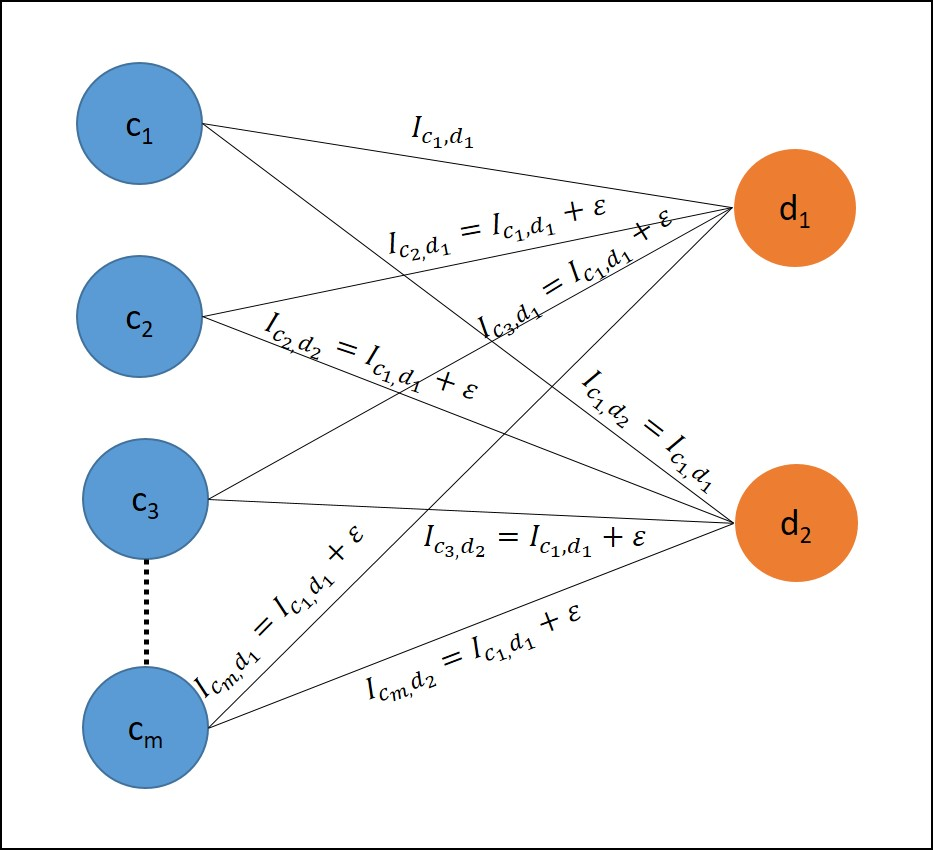
\includegraphics[width=\linewidth]{Graph/badExample1.jpg}
\caption{An in-feasible solution by MIKIRA}
\label{fig:bad1}
\end{subfigure}
\begin{subfigure}{0.32\linewidth}
\centering
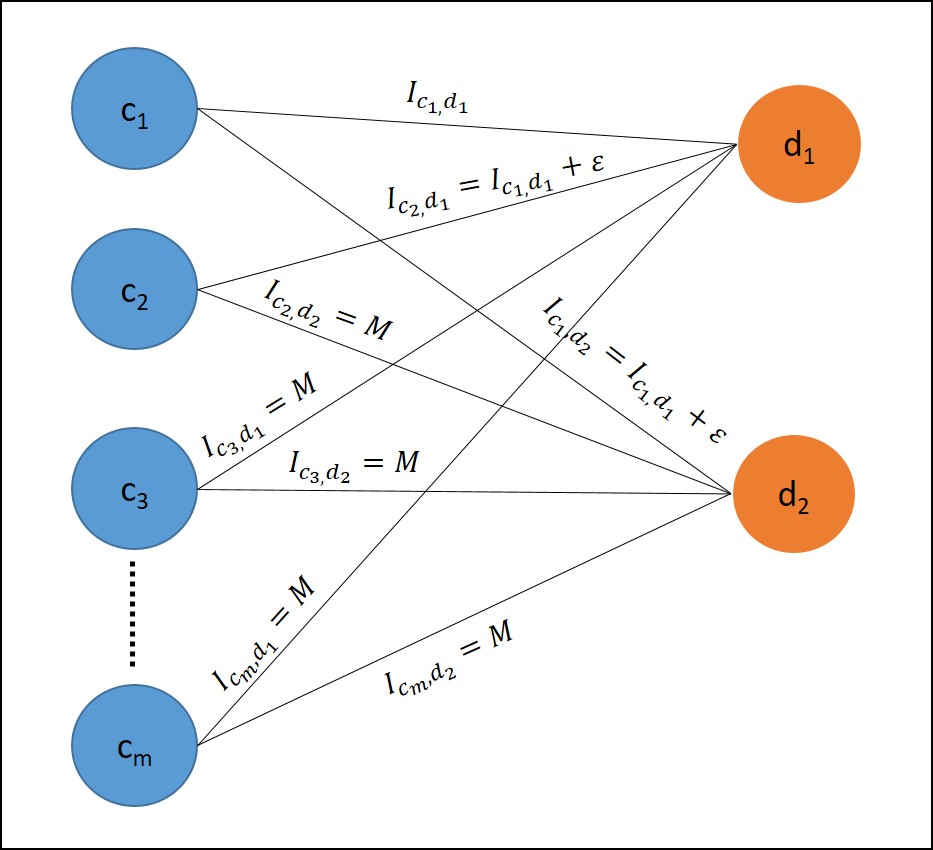
\includegraphics[width=\linewidth]{Graph/badExample2.jpg}
\caption{An unbounded solution by TAFIRA}
\label{fig:bad2}
\end{subfigure}
\begin{subfigure}{0.32\linewidth}
\centering
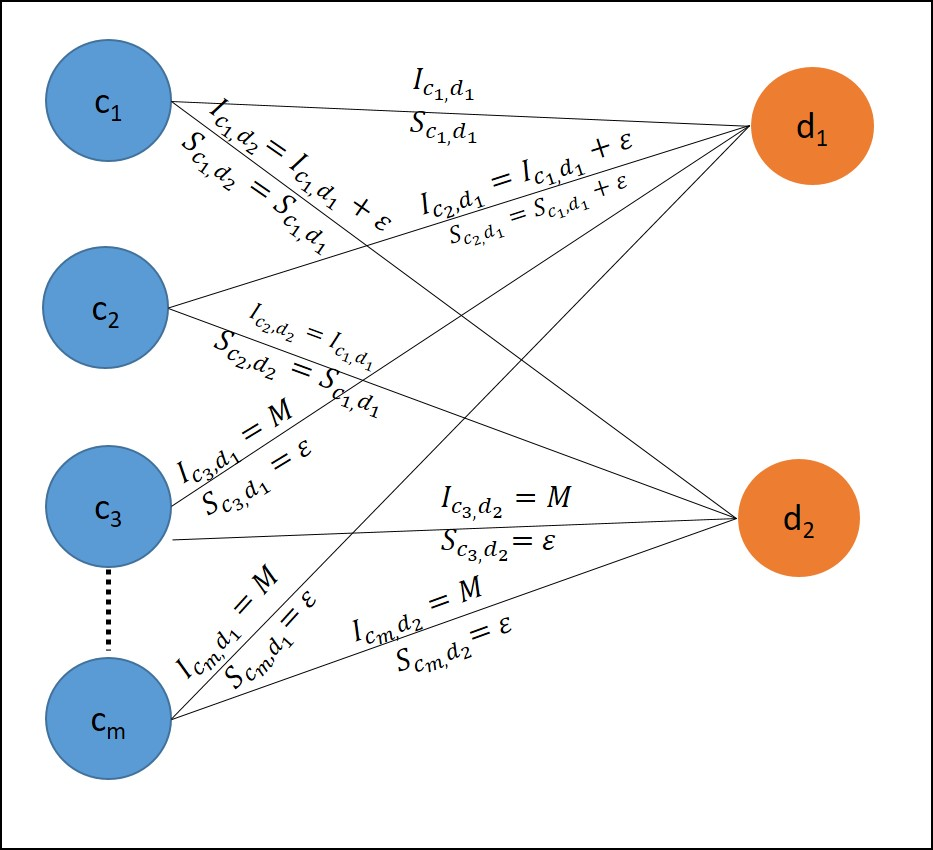
\includegraphics[width=\linewidth]{Graph/badExample3.jpg}
\caption{A failed case of TAFIRA}
\label{fig:bad3}
\end{subfigure}
}
}%
\caption{Worst cases of TAFIRA and MIKIRA}
\end{figure*}


\smallskip
 
A two phase auction based fair resource allocation algorithm (TAFIRA) \cite{islam2016radio} also considers the same problem we are considering. TAFIRA minimizes the interference while achieving the system sum rate demand by allocating all D2D pairs to the available cellular UEs. In Phase-I, TAFIRA creates a bidding pool with all cellular UEs and a set of bidders with all D2D pairs. Each bidder has a greedy choice to bid for the cellular UE that produces minimum interference calculated from (\ref{eqn:interference}). Once all D2D pairs are allocated to cellular UEs, the algorithm calculates the total system sum rate according to the allocation. If the calculated system sum rate satisfies the sum rate demand $T$ according to (\ref{eqn:constrain_target}), then TAFIRA terminates and reports the allocation as the final result. But if the demand is not satisfied in Phase-I, TAFIRA goes to Phase-II with the result provided in Phase-I where it releases a D2D pair and allocates it to any of the unallocated cellular UEs only if it improves the system sum rate. If TAFIRA fails to meet the sum rate demand in Phase-II, it reports that the allocation satisfying sum rate demand is not possible. Though TAFIRA can provide good solutions in average cases, the performance of the algorithm can be unbounded in the worst cases. Moreover, TAFIRA can return no solution even though a solution exists.

\smallskip

 \textbf{\textit{Theorem $5.2$:}} The performance ratio of the TAFIRA, in the worst case, is unbounded. \\
 \textbf{\textit{Proof}}:  The performance ratio of an algorithm indicates the ratio between the solution given by this algorithm and the optimal solution. In this paper the performance ratio represent the ratio of induced interference by the proposed algorithm and optimal solution. Consider figure~\ref{fig:bad2}  where an edge between a cellular UEs ($c_i$) and a D2D pair ($d_j$) represents the interference ($I_{c_i,d_j}$) introduced if $d_j$ is shared with $c_i$  (M is a very large positive number, $\epsilon$ is a very small positive number and $I_{c_1,d_1}$ is the smallest component among all). Now if we consider the target sum rate R, as 0 (any sum rate suffices as long as we can minimize the total interference) then TAFIRA returns the total minimum interference as $M+I_{c_1,d_1}$ (by sharing $c_1$ with $d_1$ and $c_2$ with $d_2$) whereas the optimal solution is $2(I_{c_1,d_1}+\epsilon)$ (by sharing $c_1$ with $d_2$ and $c_2$ with $d_1$). So the performance ratio of TAFIRA is unbounded (depends on the value of M).
 
\smallskip

 \textbf{\textit{Theorem $5.3$:}} TAFIRA can return no solution for an instance even though a solution exists.\\
 \textbf{\textit{Proof}}: Consider a similar example in figure~\ref{fig:bad3} that also represents the system sum rates (sum rate contributions by any $c_i$ and $d_j$ due to sharing). It is to be noted that, sum rate does not depend only on the interference (\ref{eqn:sinr_enb}). Now, for this instance, TAFIRA gives total interference $2 \times I_{c_1, d_1}$, (by sharing $c_1$ with $d_1$ and $c_2$ with $d_2$) with total sum rate $2 \times S_{c_1, d_1}$, at the end of Phase-I of the algorithm. However, if the target sum rate (R) is $2(S_{c_1, d_1}+\epsilon)$, this solution is not feasible at the end of Phase-I.  Even in Phase-II, the algorithm can not improve the system sum rate from $2 \times S_{c_1, d_1}$.  Hence, TAFIRA can not provide any solution for this instance. However, there exists a solution (optimal) which shares $c_1$ with $d_2$ and $c_2$ with $d_1$ (total interference is $2(I_{c_1, d_1}+\epsilon$) and the total sum rate is exactly the same as target sum rate which is $2(S_{c_1, d_1}+\epsilon)$).


\section{Proposed Algorithm}\label{section:algorithm}
\smallskip
 
Resource allocation problem in D2D communication can be converted into a weighted bipartite matching problem. We propose a resource allocation algorithm for both the fair (FARA) and restricted (RARA) assignment by using weighted bipartite matching approach. Formation of the bipartite graph, weight calculation of the bipartite graph and proposed resource allocation algorithm is discussed in the following subsections.

\subsection{Formation of the bipartite graph} \label{subsection:Formation of Bipartite Graph}
\smallskip
 
The bipartite graph is constituted of two disjoint sets, i) set of existing cellular UEs $C$ and ii) set of D2D pairs $D$. 

\subsection{Weight calculation} \label{subsection:Weight Calculation}
\smallskip
 
We consider cellular UEs $C(c_1,c_2,\ldots, c_n)$ and D2D pairs $D(d_1,d_2,\ldots,d_m)$ as the two sets of vertices of the weighted bipartite matching problem where the edges between $c_i$ and $d_j$ represent the interference and sum rate introduced due to the sharing of RBs between $c_i$ and $d_j$. The weight of the edges is crucial to find the best matching. Initially, our algorithm runs weighted bipartite matching algorithm \cite{hungarian} to find the possible minimum system interference by sharing RBs among the set of cellular UEs  and the set of D2D pairs. Later, our algorithm may need to find the possible maximum system sum rate for the same setting.

\smallskip
 
We introduce a $n \times n$ matrix $Y$ as the weight matrix for the weighted bipartite matching algorithm (which represents the edges) where rows represent the cellular UEs and columns represent the D2D pairs. As weighted bipartite matching algorithm deals with only square matrix, we add $(n-m)$ dummy D2D pairs in the weight matrix. In case of FARA, first $m$ columns of $Y$ holds the interference caused by $c_i$ and $d_j$ using (\ref{eqn:interference}) and we assigned $0$ to the remaining $(n-m)$ dummy D2D pairs as we do not want them to be matched in the final solution. On the other hand, in case of RARA, if sharing RBs of $c_i$ with $d_j$ decreases the system sum rate, then  we assigned $0$ to that edge as we also do not want them to be matched in the final solution. 
 
\smallskip
 
Similarly, for sum rate maximization, we need to calculate the input weight matrix for the weighted bipartite matching algorithm. A $n \times n$ matrix $X$ (similar to matrix $Y$) is introduced for this matching algorithm. Here, in case of FARA, weight for first $m$ columns is the system sum rate contributed by $c_i$ and $d_j$ using (\ref{eqn:sumrate}). However, for remaining $(n-m)$ dummy D2D pairs, the weight is calculated by using (\ref{eqn:sumrate_0}), which ensures that dummy D2D pairs do not affect the selection of actual D2D pairs. In case of RARA, if sharing RBs of $c_i$ with $d_j$ decreases the system sum rate, then we assign the value of the sum rate obtained for $c_i$ by using (\ref{eqn:sumrate_0}) to that edge as we do not want them to be matched in the final solution too.

\smallskip

It should be noted that, if any system demands then QoS constraint for any individual cellular UE and D2D pair can be applied at the time of calculating weight of the edges. Weight $infinity (\infty)$ is set to those edges which do not satisfy predefined SINR constraints. This can force the algorithm to avoid this type of sharing.
  
\subsection{Interference Minimization Resource allocation algorithm}\label{section:FairAssignment}
\smallskip
 
We translate the resource allocation problem that we are addressing in this paper, into a weighted bipartite matching problem. Here, for the fair assignment, each D2D pair needs to be assigned to exactly one cellular UE (\ref{eqn:constraintFair}) and for the restricted assignment a D2D pair shares RBs of maximum one cellular UE or it can remain unassigned (\ref{eqn:constraintRestricted}). The goal of the assignment is to attain minimum interference while maintaining a target system sum rate $T$. This paper provides a two phase resource allocation algorithm for both fair and restricted assignment to solve this problem. The inputs of our algorithm is a set of cellular UEs $C$, a set of D2D pairs $D$, target system sum rate $T$. In phase-I (Assignment Phase) of our algorithm, a weighted bipartite matching approach is used to get an initial solution for the resource allocation problem. In this phase,  the only difference between $FARA$ or $RARA$  is in weight calculation. The process of weight calculation is discussed in subsection \ref{subsection:Weight Calculation}. In phase-II (Improvement Phase) of the proposed algorithm, local search techniques are used to improve the solution of assignment phase (Phase-I). The following subsections describe the phase-I and phase-II of the proposed algorithm. 


\begin{algorithm}

   \caption{Phase-I (Assignment Phase)}
   \label{algorithm1}
    \begin{algorithmic}[1]
    \footnotesize
    \Procedure{PHASE-I}{$C(c_1,c_2,\ldots, c_n),D(d_1,d_2,\ldots,d_m),T$}
    \Comment{An allocation from $C$ to $D$, $T$ is the target system sum rate}
        \State Let $X[n][n], Y[n][n]$ be two new weight Matrices \label{algorithm1:interferenceMatrix}
        \Comment{$X_{i,j}, Y_{i,j}$ is the sum rate and interference respectively when $d_j$ shares RBs of $c_i$}
        
        \State Calculate interference weight matrix $Y$ for preferred assignment (FARA or RARA)
	
	\State $Z = \textproc{HungarianMin}($Y$)$  \Comment using (\ref{eqn:sumrate_total}) \label{algorithm1:hung_min}
	
	\If{$Z \geqslant T$}\;\label{algorithm1:checkreturn1}
		\State Allocate RBs of $c_i$ to $d_j$ for all $TRUE$ value of $M_{i,j}$
		\State \textbf{Return Current Allocation.}\Comment Optimal solution
	\Else\Comment{Phase-I failed}
		
				
			\State Calculate sum rate weight matrix $X$ for preferred assignment (FARA or RARA)

		\If{$T >  \textproc{HungarianMax}($X$)$}\label{algorithm1:checkispossible}
			\State \textbf{Allocation satisfying $T$ is not possible.}
		\Else
			\State Allocate RBs of $c_i$ to $d_j$ using \textproc{HungarianMax}($X$) 
			\If {$assignment$ is $fair$}
			\State Go to \textproc{Local Search (FARA-II)}
			\EndIf
			\If {$assignment$ is $restricted$}
			\State Go to \textproc{Local Search (RARA-II)}
			\EndIf
		\EndIf 
				
	\EndIf 
\EndProcedure
\vspace{-0.1cm}
\end{algorithmic}
\end{algorithm}


\subsubsection{Phase-I (Assignment Phase) of FARA and RARA}
\smallskip
 
Initially, we run Hungarian minimization algorithm \cite{hungarian} (minimum weighted bipartite matching algorithm) to find the possible minimum total system interference by sharing RBs among a set of cellular UEs $C(c_1,c_2,\ldots, c_n)$ and a set of D2D pairs $D(d_1,d_2,\ldots,d_m)$. We consider $C$ and $D$ as the two sets of vertices of the matching problem where the edges between $c_i \in C $ and $d_j \in D$ represent the interference, $I_{c_i,d_j}$ introduced due to the sharing of RBs between $c_i$ and $d_j$. We introduce a $n \times n$ matrix $X$ and $Y$ in line \ref{algorithm1:interferenceMatrix} of algorithm \ref{algorithm1} and the calculation of their value is discussed in subsection \ref{subsection:Weight Calculation}. The matrix $Y$ is the interference weight matrix and weights are assigned based on the algorithm selected (FARA or RARA). The Hungarian algorithm assigns D2D pairs to cellular UEs (line \ref{algorithm1:hung_min} of algorithm \ref{algorithm1}) and returns the corresponding system sum rate $Z$. If the system sum rate meets the target sum rate $T$ (line \ref{algorithm1:checkreturn1} of algorithm \ref{algorithm1}), then we consider this allocation as the optimal solution of the resource allocation problem. However, if the result of this minimization bipartite matching fails to surpass the target sum rate then we use Hungarian maximization algorithm (maximum weighted bipartite matching algorithm) to find the possible maximum system sum rate for the same instance of the problem to check whether there exists any solution or not.  Please note that we can do this checking at the start of the algorithm. However, we prefer this step later as we use the result of this step in the Phase-II of the algorithm. Line \ref{algorithm1:checkispossible} of algorithm \ref{algorithm1} solves the maximum bipartite matching problem which gives the optimal system sum rate. The matrix $X$ is the sum rate weight matrix for Hungarian maximization and weights are calculated based on the selected assignment types (FARA or RARA). Therefore, based on the assignment type, Hungarian maximization returns the maximum possible system sum rate (which is optimal). If the target sum rate is greater than calculated optimal system sum rate (line \ref{algorithm1:checkispossible} of algorithm \ref{algorithm1}), then we can confirm that there exists no solution for the current instance of the allocation problem. However, if the target sum rate is lower than or equal to the calculated sum rate then we consider current allocation as a candidate solution.  Phase-II of our algorithm is a local search technique, that takes this initial feasible solution and tries to minimize the total interference iteratively until it reaches the local optima. 

\begin{algorithm}
   \caption{Phase-II (Improvement Phase) for FARA}
   \label{algorthm2}
    \begin{algorithmic}[1]
    \footnotesize
    \Procedure{FARA-II}{}
%    \Comment{An allocation from C to D}
   % \State $improvement = TRUE$
   \State Calculate current system interference
	\While{$improve$}\label{algorithm2:while}
   		\For{ each pair $(c_i,c_j) \in C$ where $i \neq j$}
   		\State $d_i$ and $d_j$ are D2D pairs assigned with $c_i$ and $c_j$ receptively
   		   \State Calculate current system sum rate $z$
   		   	\If{ $I_{c_i,d_j} + I_{c_j,d_i} < I_{c_i,d_i} + I_{c_j,d_j} $ and $z-S_{c_i,d_i}-S_{c_j,d_j} + S_{c_i,d_j}+S_{c_j,d_i} \geqslant T$  } \Comment{Swapping} \label{algorithm2:lower interference}	
   					\State Remove RBs of $c_i$ from $d_i$ and assign those RBs to $d_j$\label{algorithm2:swap}
   					\State Remove RBs of $c_j$ from $d_j$ and assign those RBs to $d_i$
   					\State Update total system interference
   					%\State $currSum = sumRate$\label{algorithm2:update sum rate}
   					
   			\EndIf 		
   		\EndFor  
  	\EndWhile\label{algorithm2:while_end}
  	\State \textbf{Return Current Allocation.}
	\EndProcedure
\end{algorithmic}
\end{algorithm}



\begin{algorithm}
   \caption{Phase-II (Improvement Phase) for RARA}
   \label{algorthm3}
    \begin{algorithmic}[1]
    \footnotesize
    \Procedure{RARA-II}{}
%    \Comment{An allocation from C to D}
   % \State $improvement = TRUE$
   \State Calculate current system interference
	\While{$improve$}\label{algorithm3:while}
   		\For{each pair $(c_i,c_j) \in C$ where $i \neq j$}
   		\State $d_i$, $d_j$ are D2D pairs assigned with $c_i$ and $c_j$ receptively   		   
   		  \State $set = \{(c_id_i,c_jd_j), (c_id_j,c_jd_i), (c_id_\phi,c_jd_i), $ 
   		  $(c_id_j,c_jd_\phi), (c_id_i,c_jd_\phi),(c_id_\phi,c_jd_j),(c_id_\phi,c_jd_\phi)\}$ 	
   		   \Comment{$c_id_j$ represents $c_i$ shares RBs with $d_j$ and $c_id_\phi$ represents $c_i$ shares RBs with no D2D pairs}	   
   		   \State Select an element from $set$ which gives lowest interference and minimize the current total interference by maintaining (\ref{eqn:constrain_target})	\label{algorithm3:lower interference}
   		   \If {such element found}
   		   		\State Allocate RBs accordingly and update total system interference
   		   \EndIf 
   		\EndFor  
  	\EndWhile\label{algorithm3:while_end}
  	\State \textbf{Return Current Allocation.}
	\EndProcedure
\end{algorithmic}
\end{algorithm}


\subsubsection{Phase-II (Improvement Phase) of FARA and RARA} \label{subsection:Improvement Phase (Phase-II)}
\smallskip
 
The goal of Phase-II is to minimize the interference while maintaining (\ref{eqn:constrain_target}). We consider two cellular users, $c_i$ and $c_j$, where $c_i$ and $c_j$ are sharing RB's with two D2D pairs $d_i$ and $d_j$ respectively. In case of FARA, we try to swap these allocations whether it can minimize the interference by maintaining the target system sum rate after this swapping (line \ref{algorithm2:lower interference} of algorithm \ref{algorthm2}). So if we can improve the solution with this swapping while maintaining the target sum rate, then we assign RBs of $c_i$ to $d_j$ and $c_j$ to $d_i$ and continue these steps until we find no such pair that can improve the solution.

\smallskip

In case of RARA, only swapping the current allocation may not improve the situation. As we have no restriction to assign all D2D pairs in this scheme, we can drop and move D2D pairs from sharing RBs. We consider all the cases for swapping, dropping and moving like 

\begin{itemize}
  \item One cellular UE can drop its D2D pair and other remain same ($(c_id_\phi,c_jd_j),(c_id_i,c_jd_\phi)$)
  \item One cellular UE can move its D2D pair to the other one and shares its RBs with no other D2D pairs ($(c_id_\phi,c_jd_i), (c_id_j,c_jd_\phi)$)
  \item Both cellular UEs can swap their assigned D2D pairs ($c_id_j,c_jd_i$)
\end{itemize}

\smallskip

We calculate the system interference and sum rate for all the cases and find the one which produces less interference as well as maintains target sum rate constraint (line \ref{algorithm3:lower interference} of algorithm \ref{algorthm3}). If such case is found, the allocation of RBs changes according to their case type. In these cases, total system interference never increases while maintaining the target system sum rate. 

\vspace{-0.1cm}

\subsection{Complexity Analysis} \label{subsection: Analysis}
\smallskip
 
The running time of the Phase-I of our algorithm is dominated by the Hungarian algorithm which is $O(n^3)$ \cite{hungarian} ($n$ is the total cellular UEs). If the total interference returned by the Phase-I of the algorithm is $W$, then the running time of the Phase-II of FARA and RARA is $O(n*m*W)$ (where m is the total D2D pairs). In the worst case we can consider that at the start of the local search the total interference is W and at the end of the local search the minimum interference value could be $0$. So, the overall running time of FARA is $O(\max(n^3, n*m*W))$ which is pseudo-polynomial in the worst case. However, we can get an $(1 - \epsilon)$ approximate solution for any local search algorithm (in our case phase-II ) in time that is a polynomial in the input size and $\frac{1}{\epsilon}$ \cite{orlin}.

\smallskip

 By analyzing the algorithm we can easily draw the following observations :

\begin {itemize}

\item The minimum weighted bipartite matching (considering interference as edge weight) among cellular UEs and D2D pairs provides the lower bound of the minimization problem (\ref{eqn:objective}).

\item If the solution of the minimum weighted bipartite matching satisfies the target system sum rate then, the proposed algorithm is optimal since the minimum weighted bipartite matching problem can be solved by using Hungarian algorithm \cite{hungarian}.

\item Total system interference never increases in the phase-II (Local Search) of the proposed algorithm while maintaining the target system sum rate (line \ref{algorithm2:while}-\ref{algorithm2:while_end} of algorithm \ref{algorthm2} and line \ref{algorithm3:while}-\ref{algorithm3:while_end} of algorithm \ref{algorthm3}).  

\item The proposed algorithm always finds the solutions if any exists (line \ref{algorithm1:hung_min}-\ref{algorithm1:checkispossible} of algorithm \ref{algorithm1}).


\end{itemize}

\section{Performance Evaluation}\label{section:FairPerformance}

\subsection{Simulation Environment}\label{sec:simulationEnvironment}
\smallskip
 
We implemented the proposed algorithm by extending NS3 (network simulator) \cite{ns3} that supports D2D communication underlaying the LTE system. We follow simulation parameters as in \cite{islam2016radio}, \cite{islam2015reducing} (Table~\ref{Simulation_table}) as well as we tune some of the parameters to check the variability of our results and we find that performance of our proposed algorithm is consistent. In our simulations, a single cell network is considered. The maximum distance allowed between the transmitter and receiver of a D2D pair is 15 meters, as some researchers assume the D2D pair to be in the same room \cite{osseiran} and a larger distance cancels the benefits gained from D2D communication. As the macro cell radius typically starts from 1000 m \cite{fujitsu}, the cell radius is chosen to be 1000 m. The target system sum rate $T$ is uniformly distributed between the system sum rate without sharing RBs with any of the D2D pairs and the maximum achievable sum rate. It should be noted that, the maximum achievable sum rate can be calculated by using the weighted bipartite matching algorithm from \cite{ccnc}. In reality the value of $T$ can be set by the network operator. We fix the total number of cellular UEs to 250 and 350, and vary the number of D2D pairs from 10 to the number of cellular UEs. Each of the simulation results presented is an average of $20$ different runs for a particular scenario. Please note that we also simulate the algorithm for various numbers of cellular UEs and the results are consistent in all the cases.

% In next subsection, the description and the performance of different other resource allocation (RA) algorithms compared to our algorithm are explained.  
 


\begin{table}[]
%to pad the row
\renewcommand{\arraystretch}{1.5}
\centering
\caption{Simulation Parameters}
\label{Simulation_table}
\begin{tabular}{|c|c|}
\hline
\textbf{Parameter}           & \textbf{Value}               \\ \hline 
Cell Radius                  & $1000$ meters                  \\ \hline
Cellular Users               & $250$                          \\ \hline
D2D pairs                    & $10$ to $250$ (increments of $10$) \\ \hline
Maximum D2D pair distance    & $15$ meters                    \\ \hline
Cellular user transmit power & $20$ dBm                       \\ \hline
D2D transmit power           & $20$ dBm                       \\ \hline
Base Station transmit power  & $46$ dBm                       \\ \hline
Noise power (AWGN)           & $-174$ dBm                     \\ \hline
Carrier Frequency            & $1.7$ GHz for LTE              \\ \hline
Bandwidth, $B$				 & $180\;$ kHz \cite{zulhasnine}	  \\ \hline
$T$				        	 & \shortstack{\\~[ Sum rate without any sharing,\\ Optimal achievable sum rate \cite{ccnc} ]}\\\hline
\end{tabular}
\end{table}



\subsection{Breakdown of the proposed algorithm}\label{Importance of Phase-II}

\begin{figure}[t]
\centering
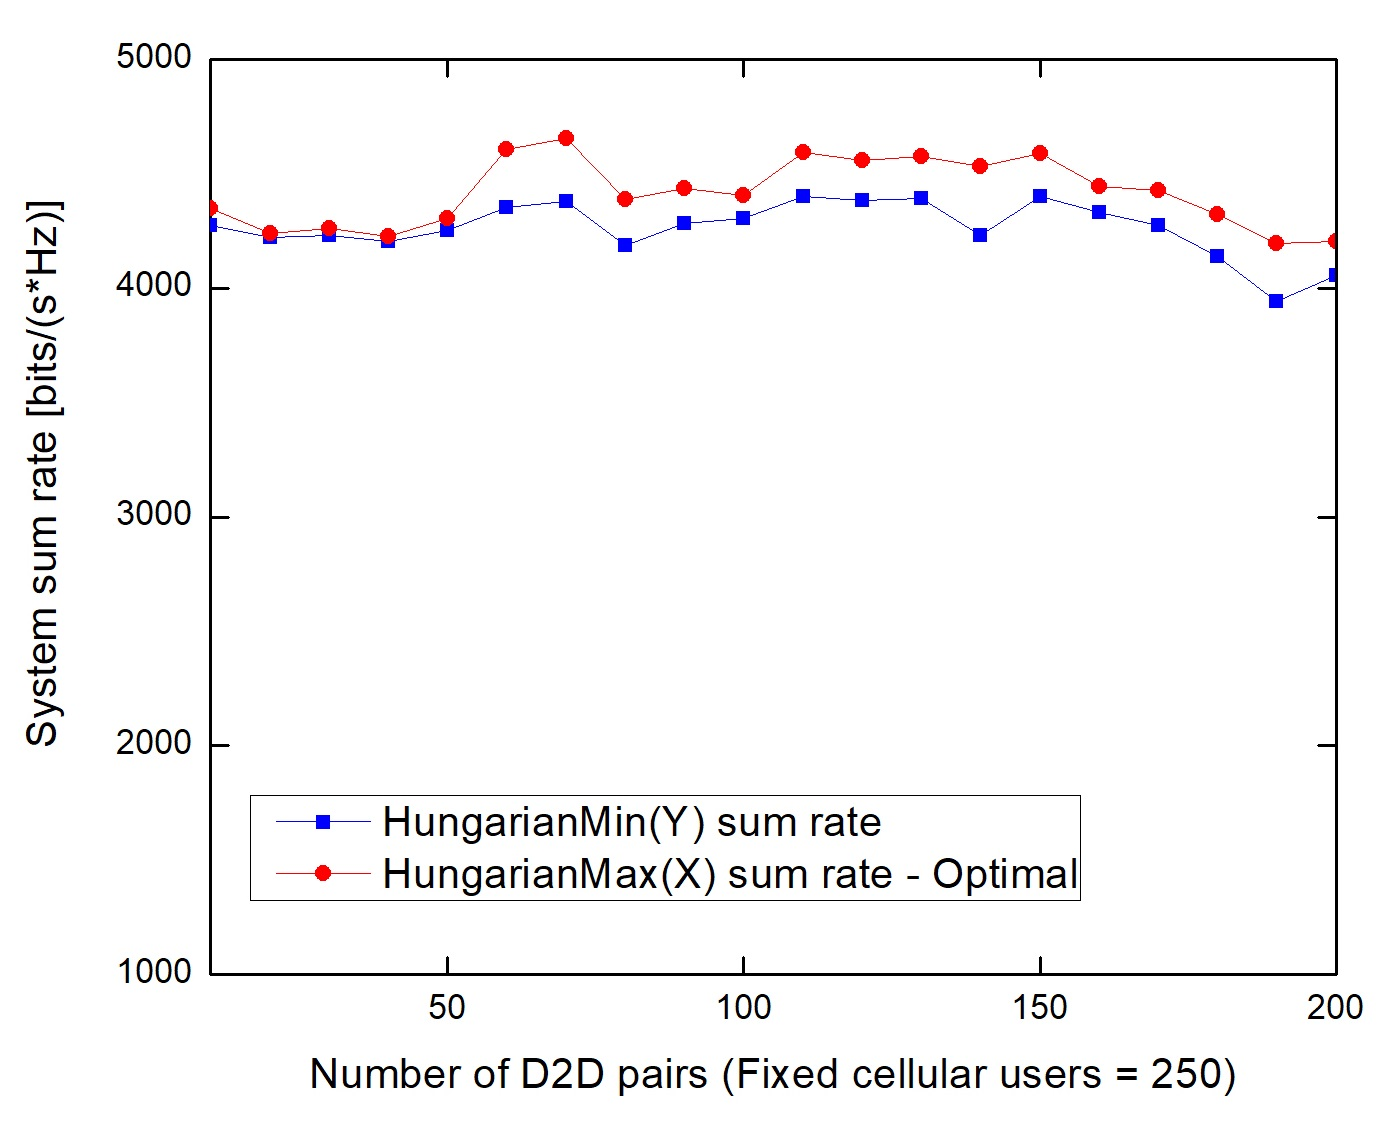
\includegraphics[width=85mm]{Graph/example_sumrate.jpg}
\caption{Total system sum rate for Hungarian minimization and maximization of Phase-I in terms of interference and sum rate respectively \label{fig:example_sum)}}
\end{figure}

\begin{figure}[t]
\centering
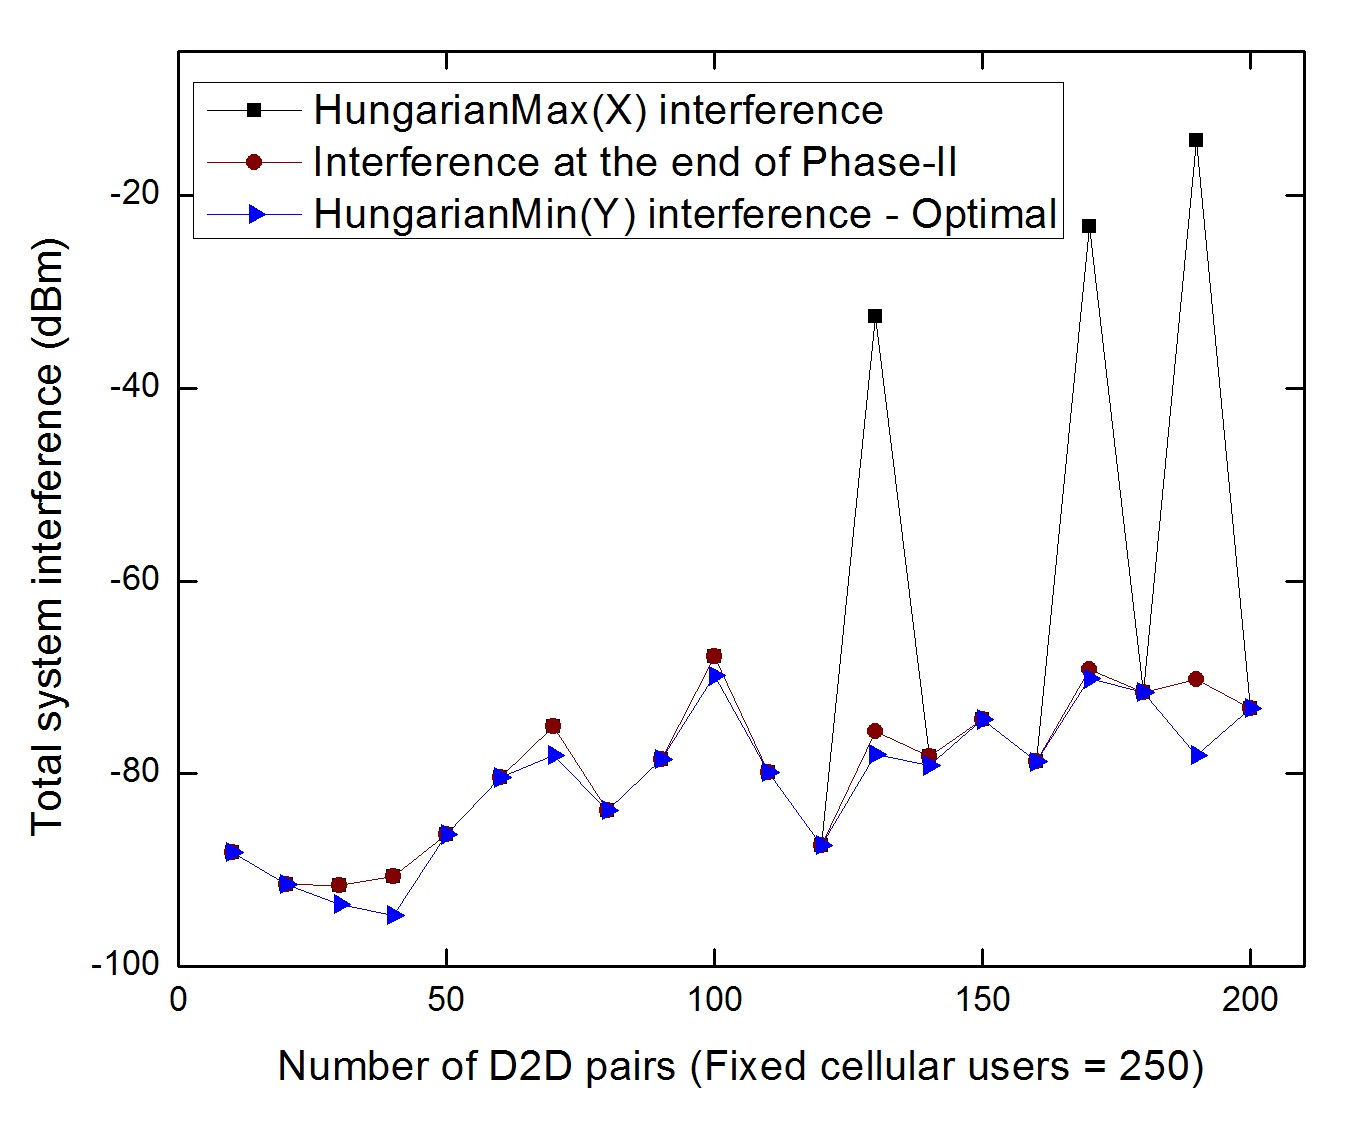
\includegraphics[width=85mm]{Graph/example_interference.jpg}
\vspace{-0.3cm}
\caption{Total system interference in different phases of FARA and RARA\label{fig:example_inter)}}
\end{figure}

\smallskip
 
In this subsection, we discuss the importance of different stages of our algorithm. At the beginning of our algorithm, we run Hungarian minimization algorithm \cite{hungarian} to find out the possible minimum system interference by sharing RBs among a set of cellular UEs and a set of D2D pairs (line \ref{algorithm1:hung_min} of algorithm \ref{algorithm1}). In figure \ref{fig:example_sum)}, blue line depicts the system sum rate achieved in line \ref{algorithm1:hung_min} of algorithm \ref{algorithm1} and red line depicts the maximum achievable system sum rate (line \ref{algorithm1:checkispossible} of  algorithm \ref{algorithm1}). If our target sum rate fits in the below of blue line, then we  get the optimal result from line \ref{algorithm1:hung_min} of algorithm \ref{algorithm1}  and execution of our algorithm is finished here. However, if our target sum rate fits to between blue and red line region, then our algorithm finds the maximum possible (optimal) system sum rate in line \ref{algorithm1:checkispossible} of algorithm \ref{algorithm1} (Hungarian maximization). After getting the optimal system sum rate, our algorithm determines whether the target sum rate is achievable or not. Our algorithm proceeds to phase-II if the target sum rate lies only in between blue and red line region, otherwise, if our target sum rate fits in the above of red line then, our algorithm confirms that no solution is possible for this instance. Thus, both Hungarian minimization and maximization operation are necessary in order to verify whether a feasible solution of the problem exists or not. Phase-II of our algorithm tries to reduce system interference generated with the assignment of phase-I while maintaining all the constraints. Hungarian maximization of sum rate in phase-I may introduce more interference in order to maximize the total system sum rate. Nevertheless, we can reduce interference from this solution as we do not need the maximized system sum rate rather  keeping total system sum rate equal or greater than the target sum rate satisfies constraint (\ref{eqn:constrain_target}). Figure \ref{fig:example_inter)} shows that our algorithm introduces more interference in phase-I and phase-II reduces interference while maintaining constraint (\ref{eqn:constrain_target}).

%\begin{figure}[t]
%\centering
%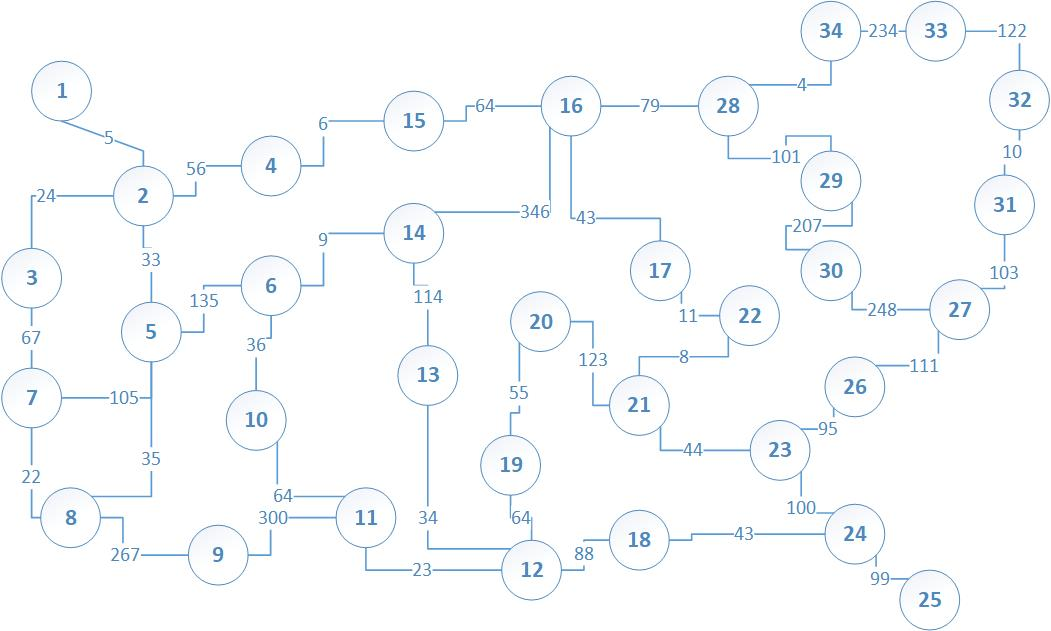
\includegraphics[width=85mm]{Graph/example.png}
%\caption{A critical scenario where the proposed algorithm reduces the interference in Phase-II \label{fig:critical_example)}}
%\end{figure}
%
%\smallskip
% 
%Now we present a scenario in figure \ref{fig:critical_example)} where phase-II of the proposed algorithm reduces the total system interference. Let us consider, $C1, C2$ and $C3$ are the cellular UEs whereas $D1$ and $D2$ are the D2D pairs. It is noted that, if any cellular UE does not share its RBs with any D2D pairs, then no interference is generated. In this scenario, we are considering FARA with a target sum rate of $12$. At the very beginning, Phase-I of the proposed algorithm applies Hungarian minimization based on the interference and calculates the assignments. Here, Hungarian minimization assigns $C1$ to $D1$, $C2$ to $D2$ and leaves $C3$ unassigned. Therefore, total system interference is $3$ and the system sum rate is $11$ which does not meet the target sum rate requirement eqn(\ref{eqn:constrain_target}). Now, both FARA and RARA apply Hungarian maximization based on the system sum rate and they assign $C3$ to $D2$, $C1$ to $D1$ and leave $C2$ unassigned. Hence, total system interference is $5$ and the system sum rate is $14$ which satisfies equation~(\ref{eqn:constrain_target}). After that, both the algorithm moves to phase-II (improvement phase) with the solution of Hungarian maximization and check if the system interference can be reduced or not. Finally, applying phase-II, we get the assignments where $C1$ shares RBs with $D2$, $C3$ shares RBs with $D1$ and $C2$ remains unassigned which reduces the interference to $4$ at the same time returns total sum rate of $12$ which satisfies the target sum rate constraint. So, in this scenario, phase-II of both FARA and RARA reduces the interference from phase-I and based on this we can conclude that phase-II our proposed algorithm reduces the system interference while maintaining all the constraints.



\subsection{Result Comparisons}\label{sec:Result Comparisons}

\begin{figure*}
{
\vspace{-15pt}
\begin{multicols}{2}
\begin{subfigure}{.86\linewidth}
 	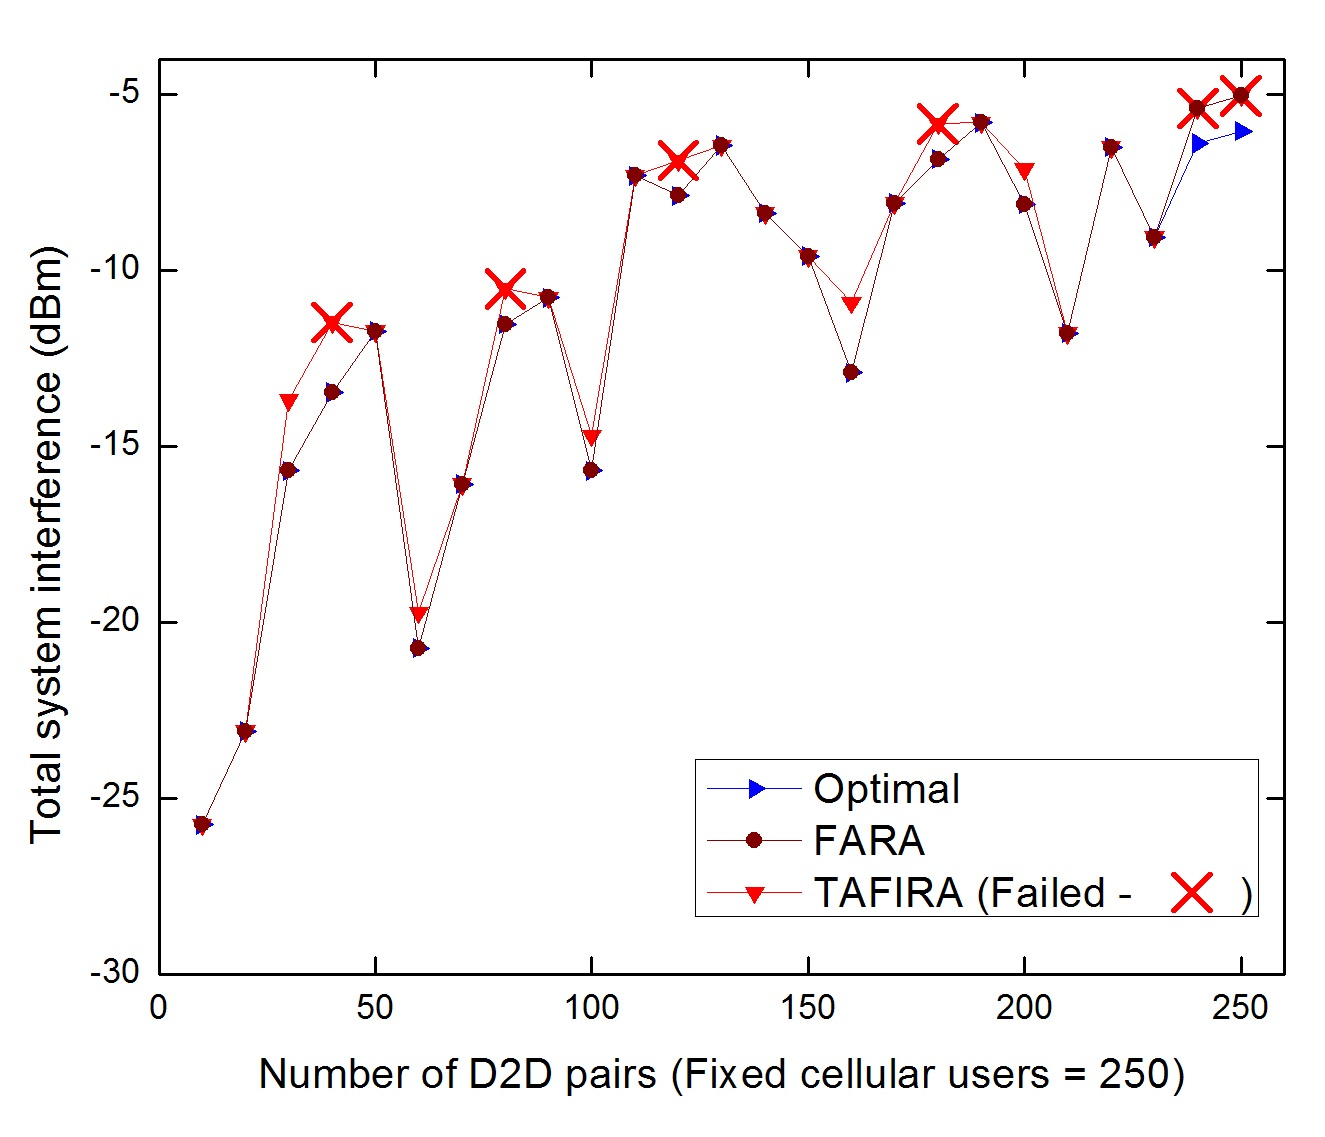
\includegraphics[width=\linewidth]{Graph/inter_fara.jpg}\par
	\caption{Comparison of total system interference}
	\label{fig:inter_fair}
	\end{subfigure}
	
	\hspace{12pt}
	\begin{subfigure}{.86\linewidth}
  	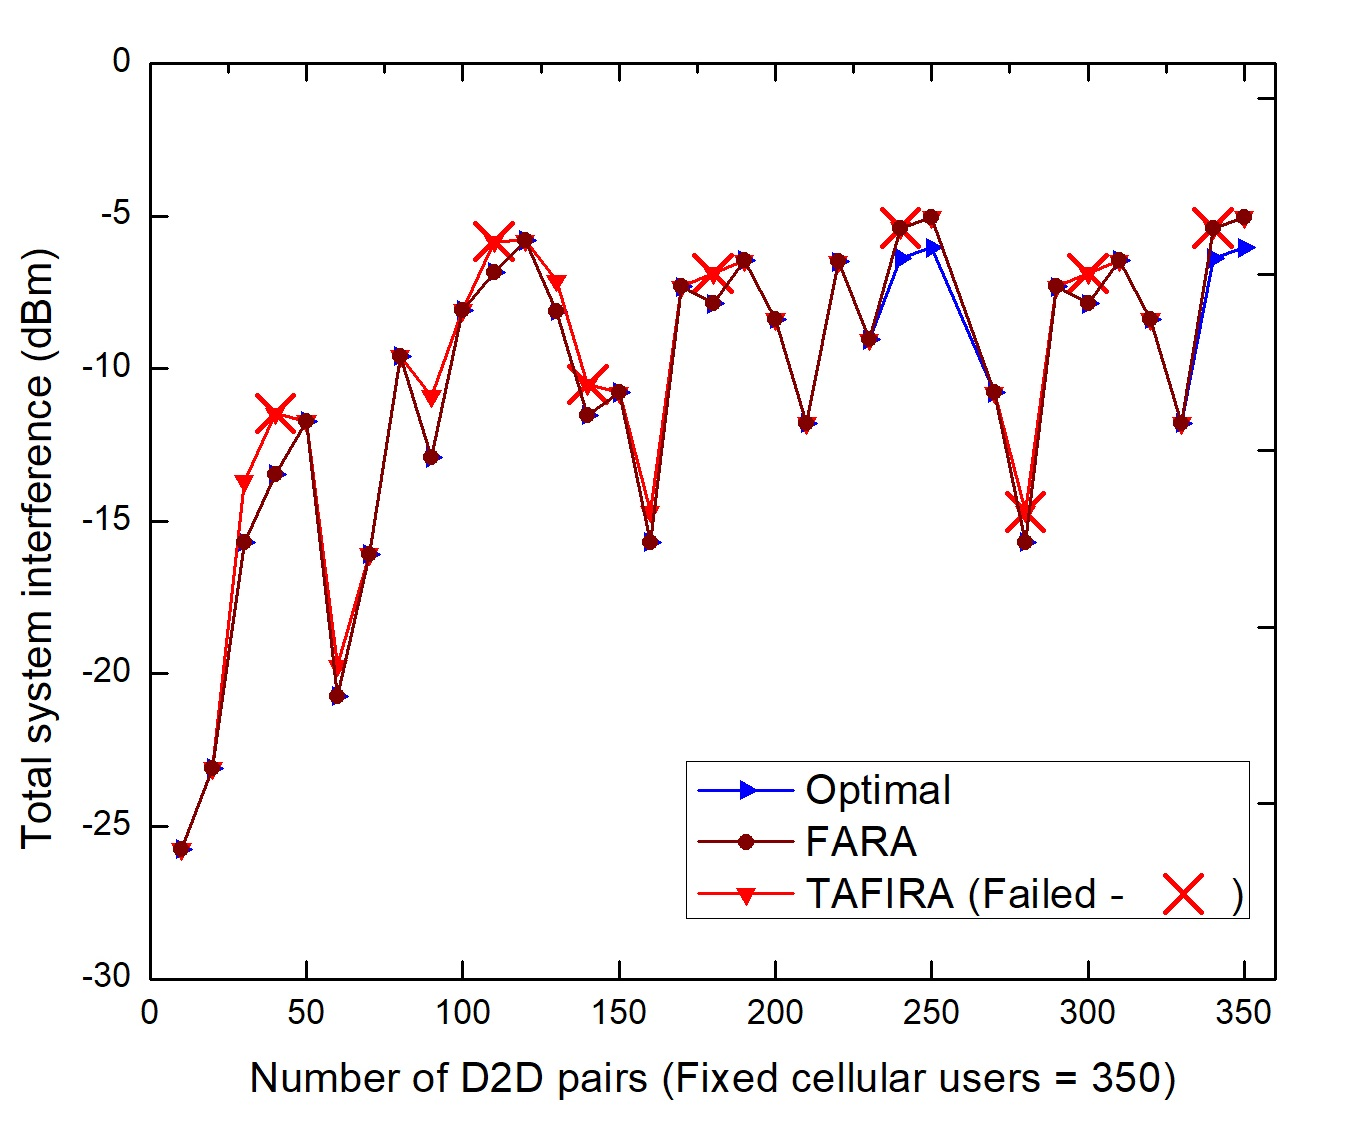
\includegraphics[width=\linewidth]{Graph/inter_fara_350.jpg}\par
	\caption{Comparison of total system interference}
	\label{fig:inter_fair_350}
	\end{subfigure}
	\end{multicols}


\begin{multicols}{2}
\begin{subfigure}{.86\linewidth}
 	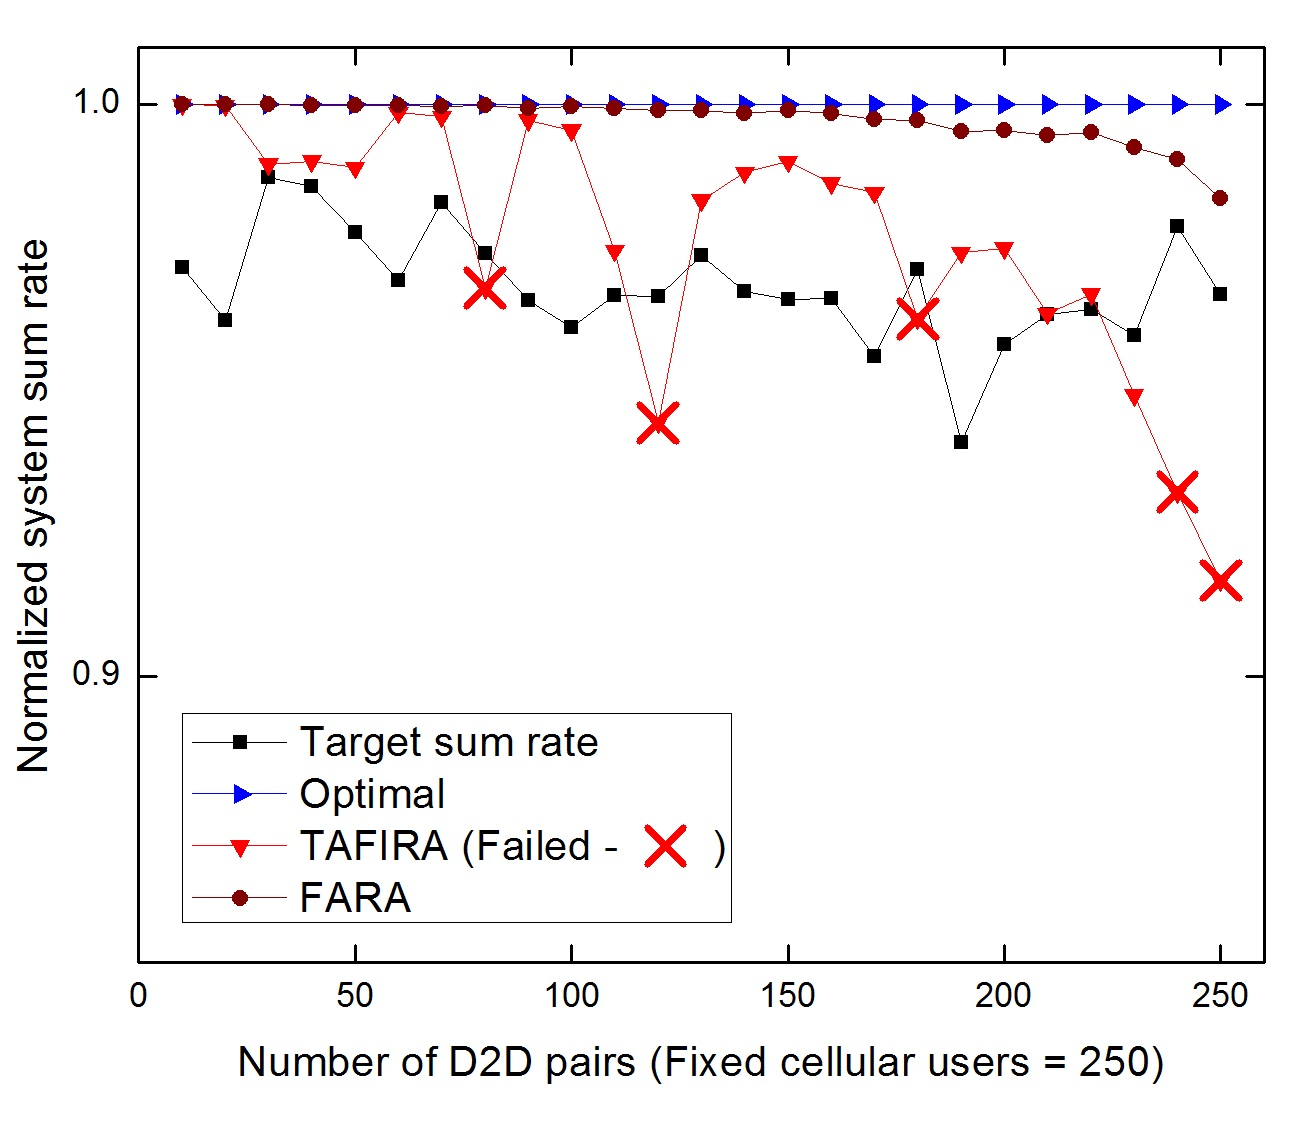
\includegraphics[width=\linewidth]{Graph/sumrate_fara.jpg}\par
	\caption{Comparison of normalized system sum rate}
	\label{fig:sumrate_fair}
	\end{subfigure}
	
	\hspace{12pt}
	\begin{subfigure}{.86\linewidth}
 	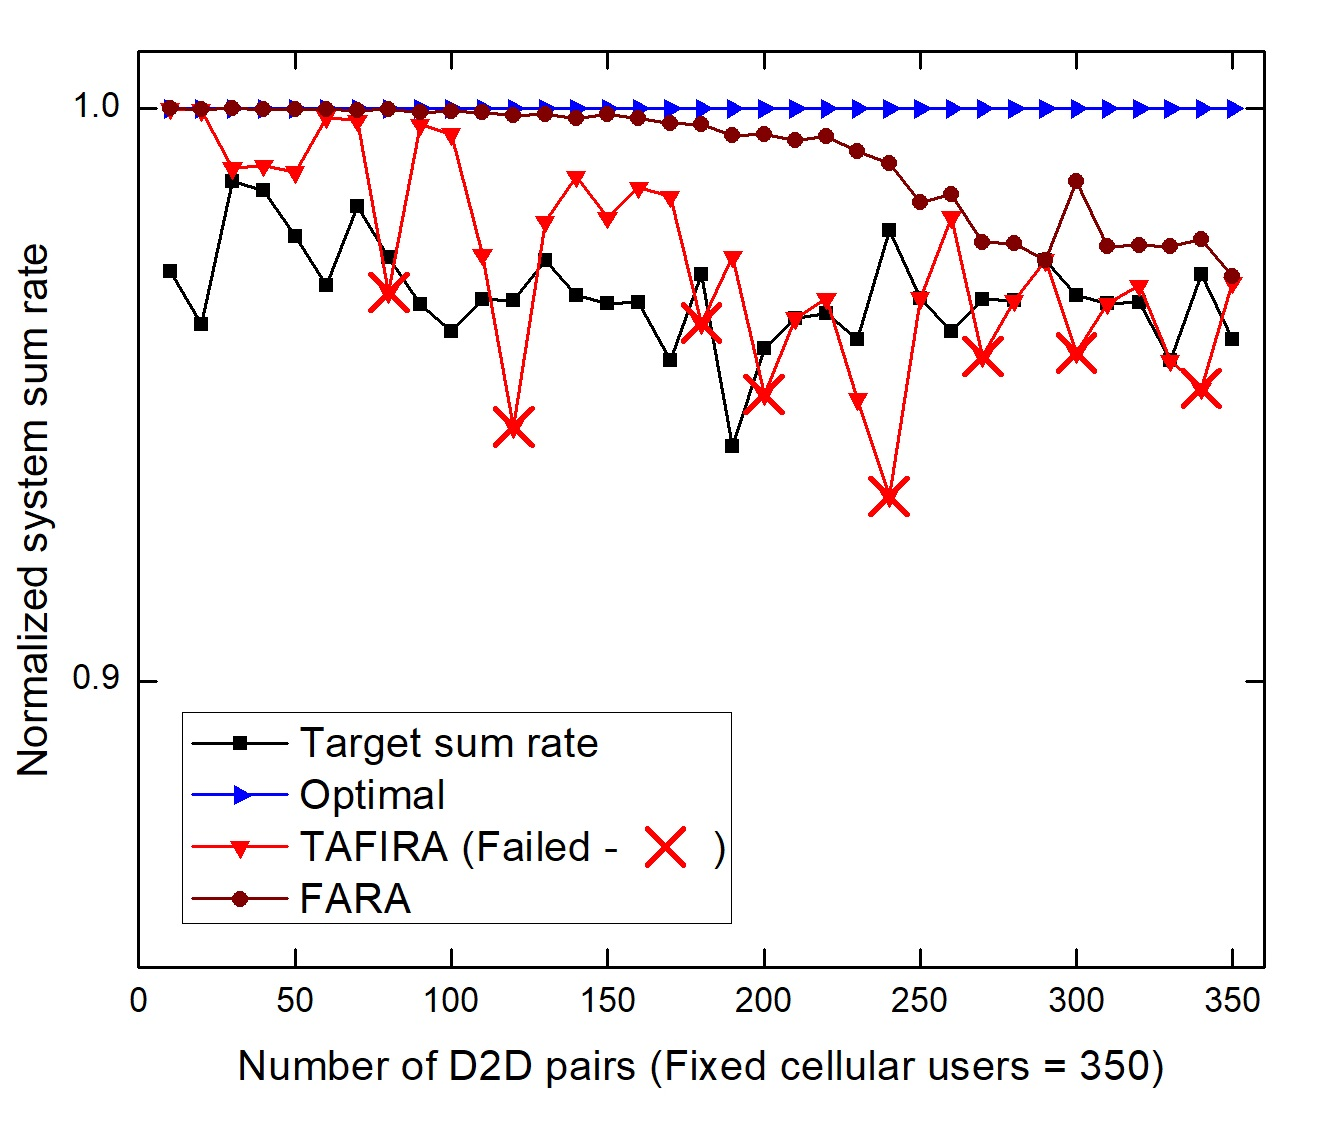
\includegraphics[width=\linewidth]{Graph/sum_fara_350.jpg}\par
	\caption{Comparison of normalized system sum rate}
	\label{fig:sumrate_fair_350}
	\end{subfigure}
	\end{multicols}

\begin{multicols}{2}
\begin{subfigure}{.86\linewidth}
	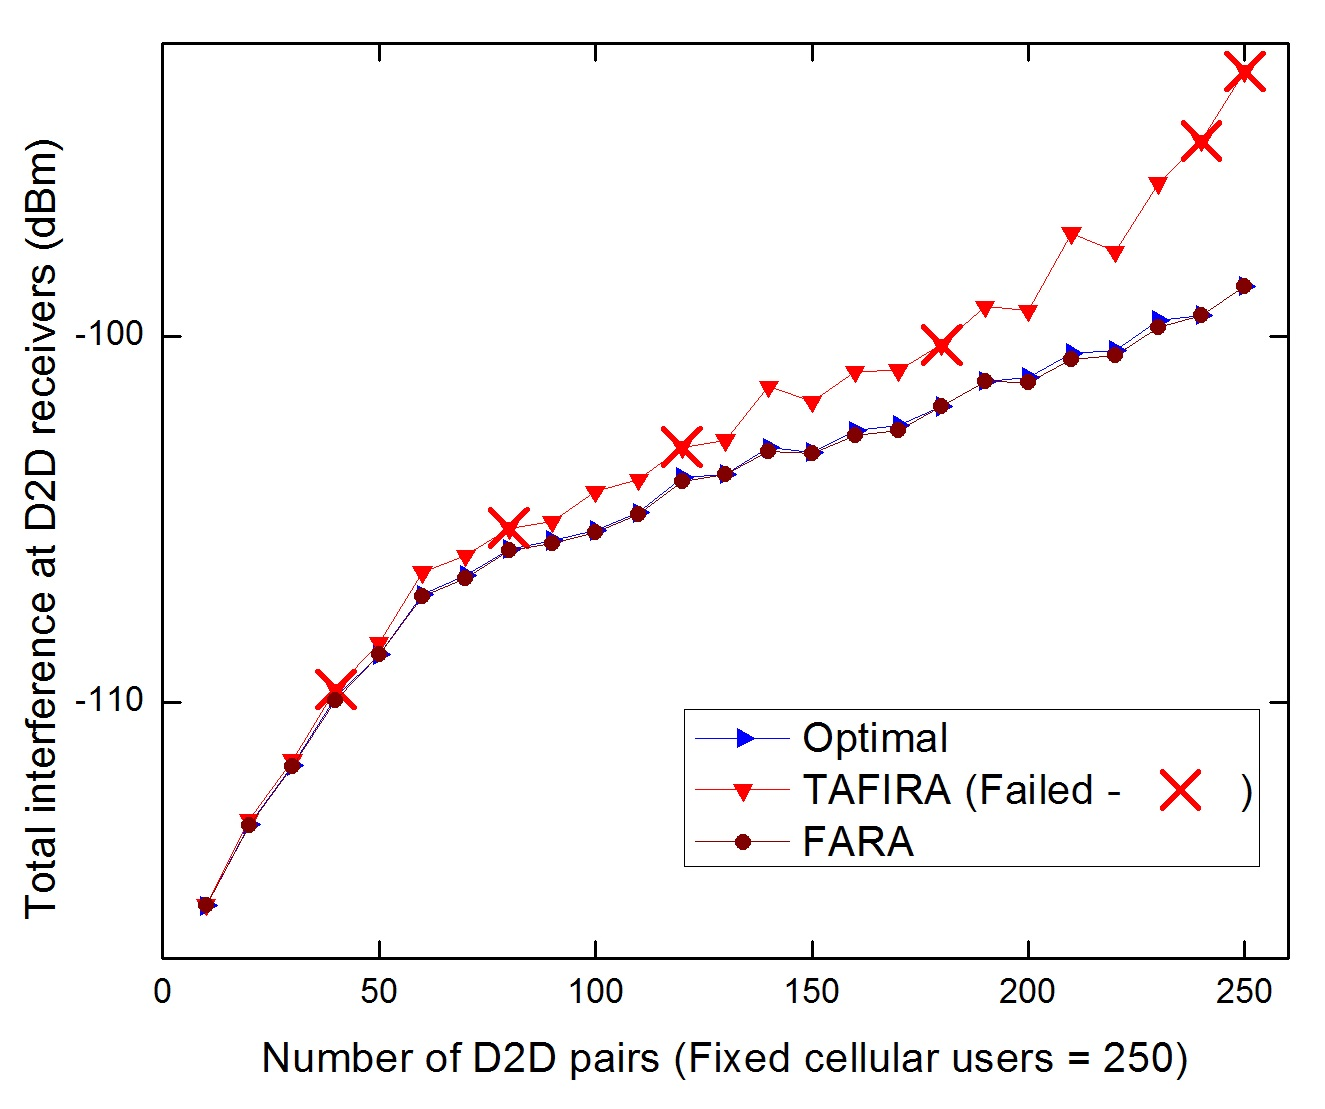
\includegraphics[width=\linewidth]{Graph/inter_d2d_fara.jpg}\par
	\caption{Comparison of total interference at the D2D receivers}
	\label{fig:inter_d2d_fair}
	\end{subfigure}
	
	\hspace{12pt}
	\begin{subfigure}{.86\linewidth}
	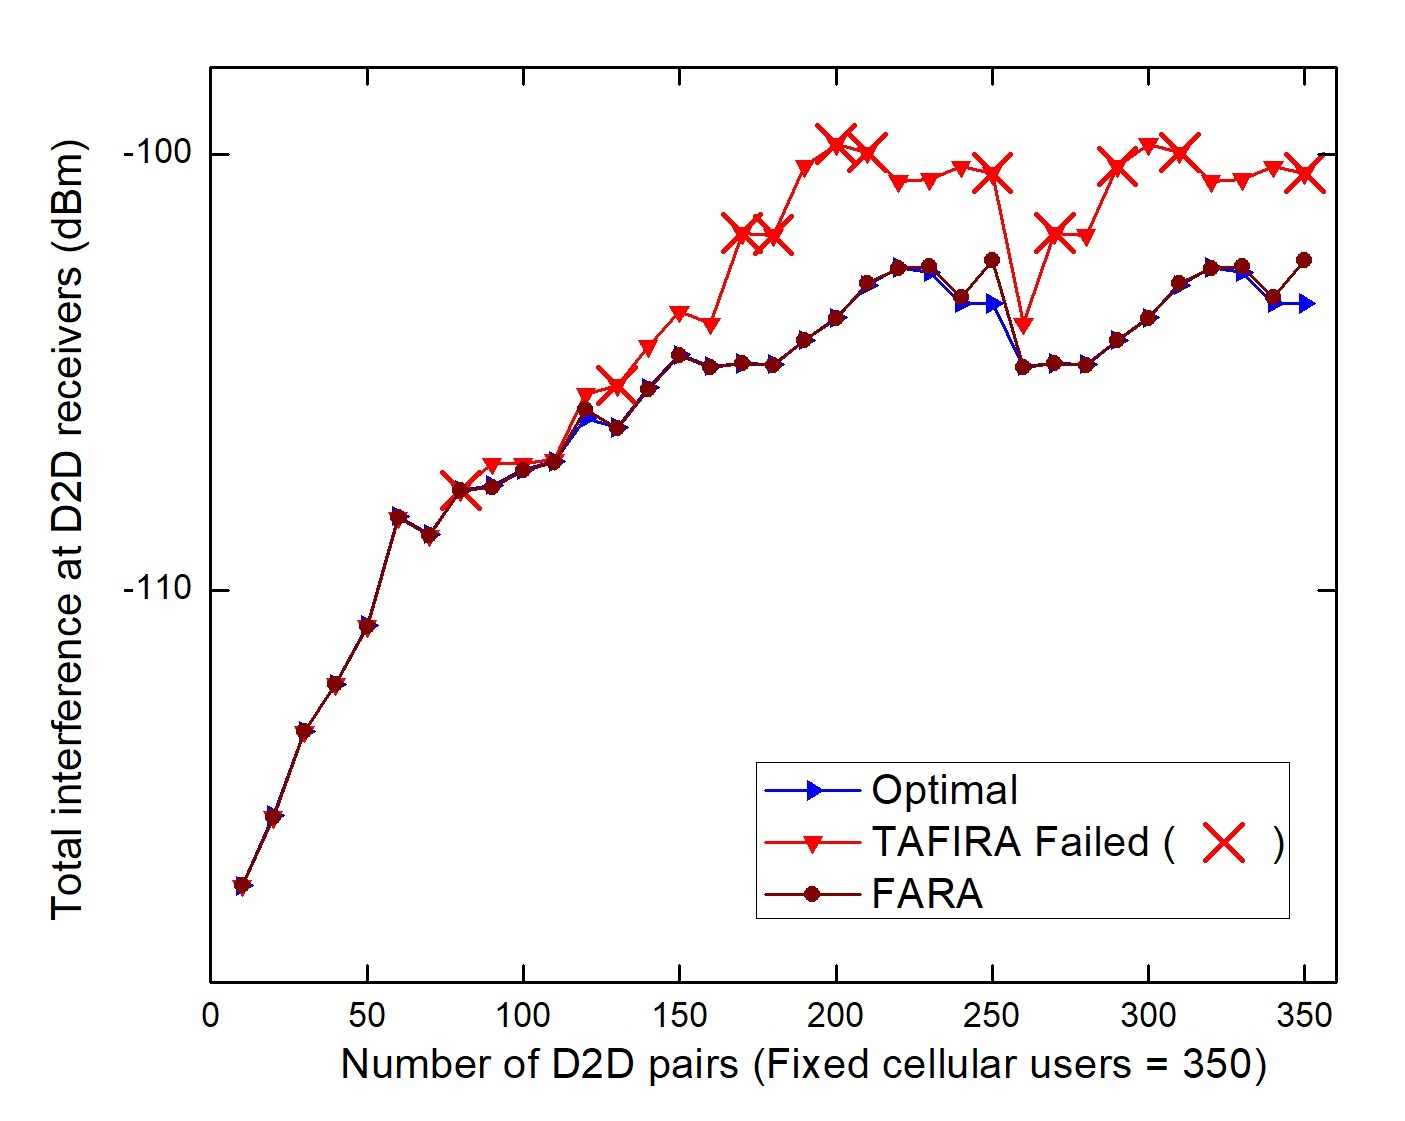
\includegraphics[width=\linewidth]{Graph/inter_d2d_fara_350.jpg}\par
	\caption{Comparison of total interference at the D2D receivers}
	\label{fig:inter_d2d_fair_350}
	\end{subfigure}
	\end{multicols}

}%
\caption{Performance comparisons among the resource allocation algorithms for fair assignment}
\label{fig:fair}
\end{figure*}


\begin{figure*}
\begin{multicols}{2}
\begin{subfigure}{.86\linewidth}
 	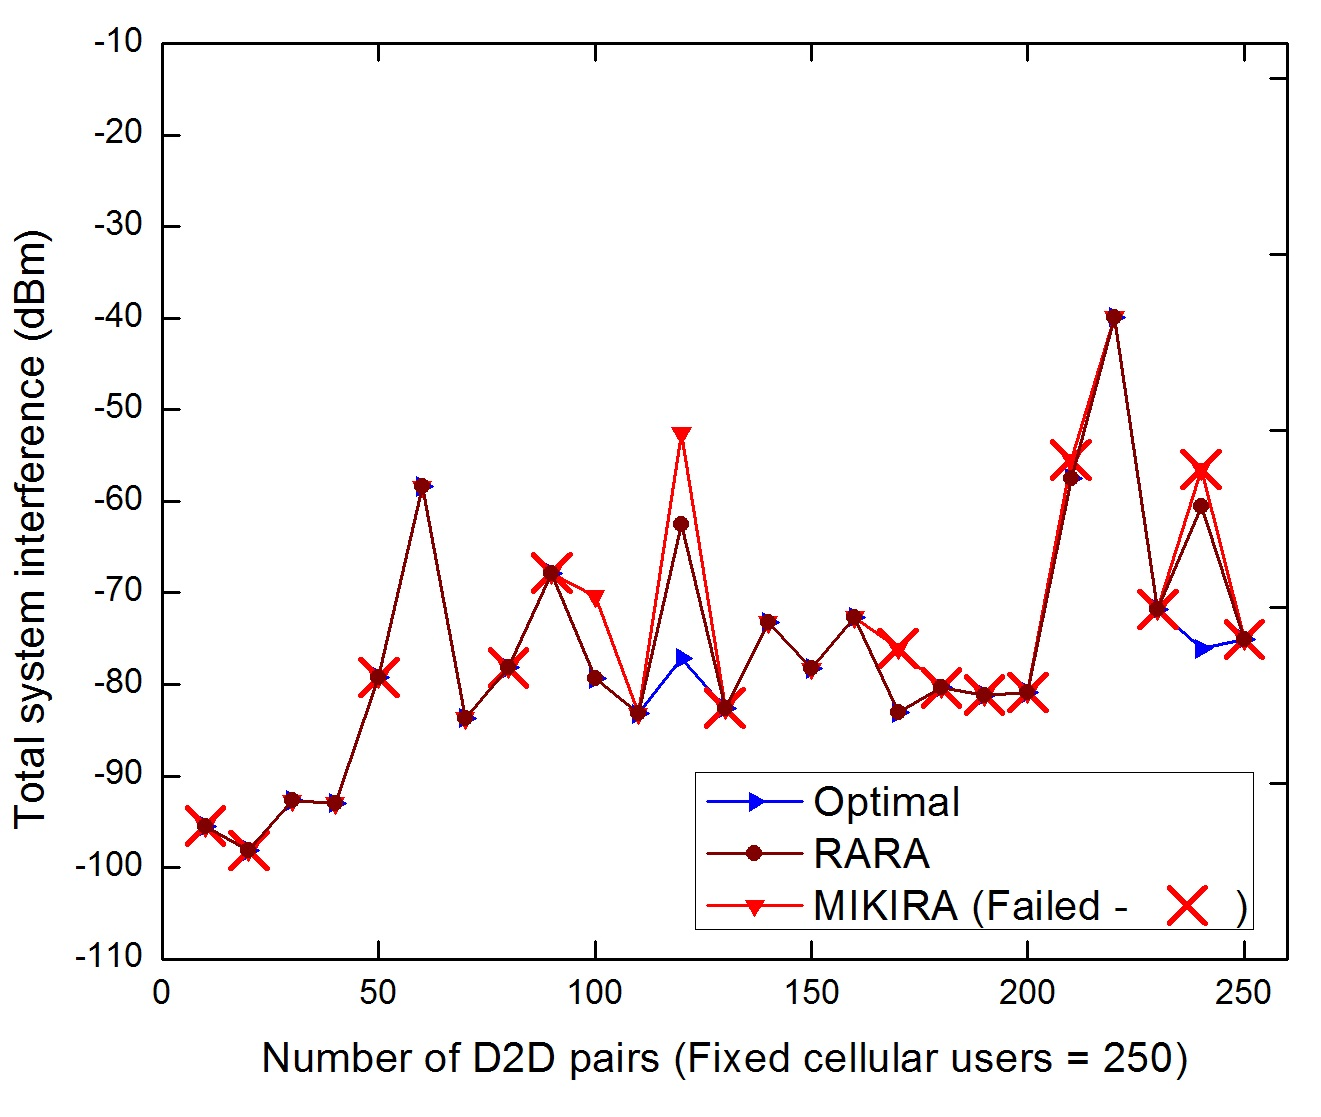
\includegraphics[width=\linewidth]{Graph/inter_rara.jpg}\par
	\caption{Comparison of total system interference}
	\label{fig:inter_res}
	\end{subfigure}
	
	\hspace{12pt}
	\begin{subfigure}{.86\linewidth}
  	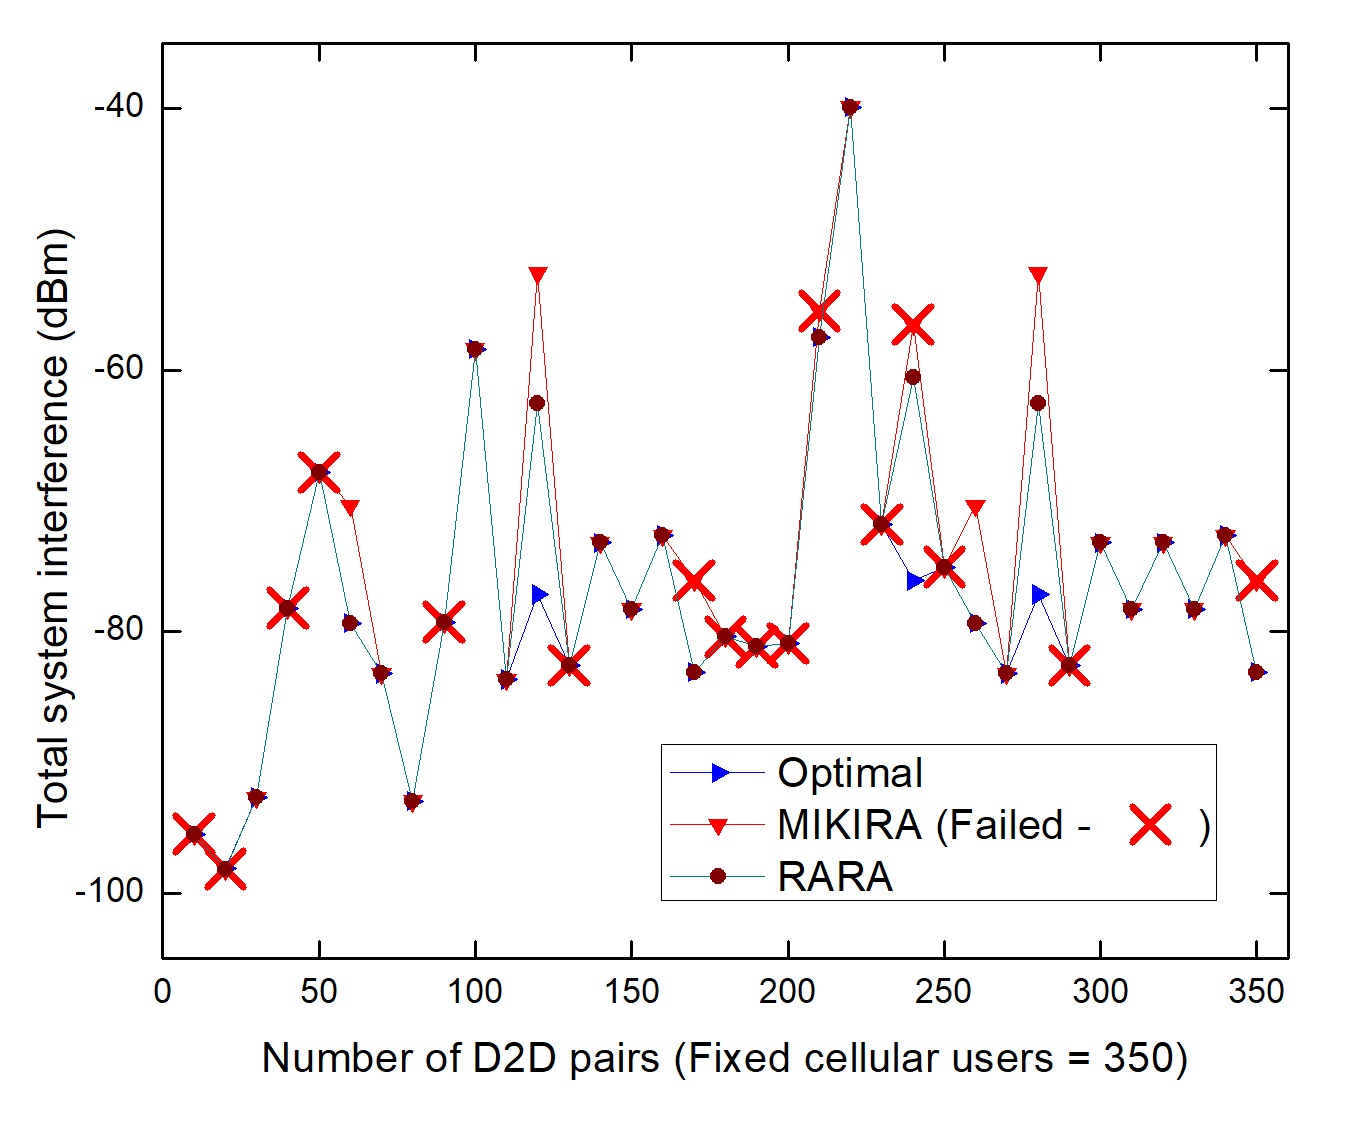
\includegraphics[width=\linewidth]{Graph/inter_rara_350.jpg}\par
	\caption{Comparison of total system interference}
	\label{fig:inter_res_350}
	\end{subfigure}
	\end{multicols}

\begin{multicols}{2}
\begin{subfigure}{.86\linewidth}
 	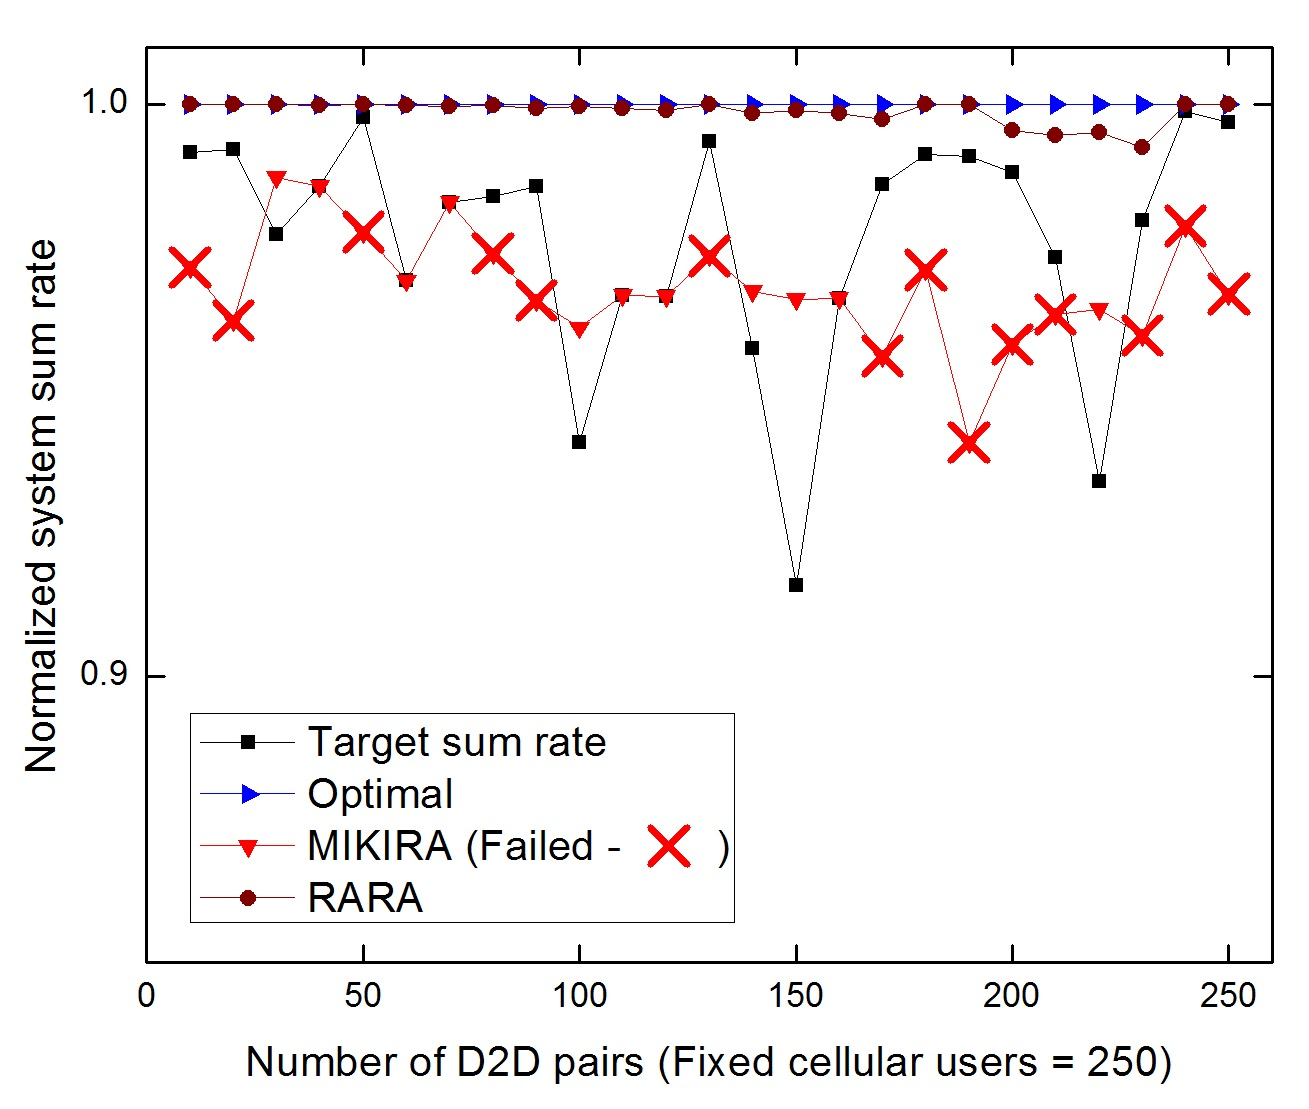
\includegraphics[width=\linewidth]{Graph/sumrate_rara.jpg}\par
	\caption{Comparison of normalized system sum rate}
	\label{fig:sumrate_res}
	\end{subfigure}
	
	\hspace{12pt}
	\begin{subfigure}{.86\linewidth}
  	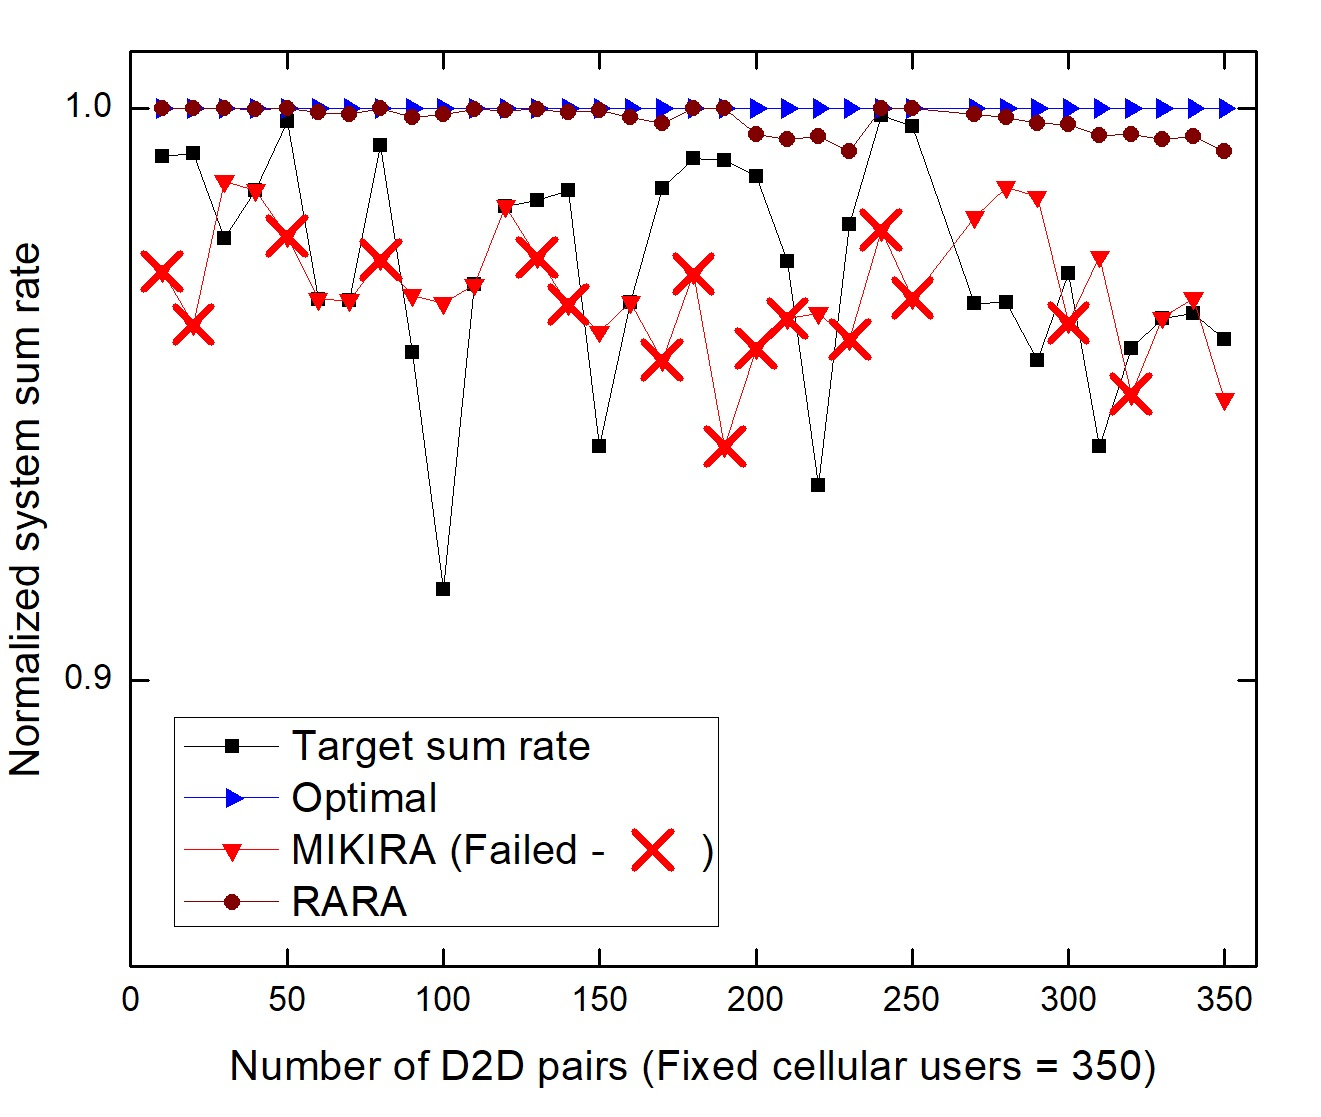
\includegraphics[width=\linewidth]{Graph/sum_rara_350.jpg}\par
	\caption{Comparison of normalized system sum rate}
	\label{fig:sumrate_res_350}
	\end{subfigure}
	\end{multicols}

\begin{multicols}{2}
\begin{subfigure}{.86\linewidth}
	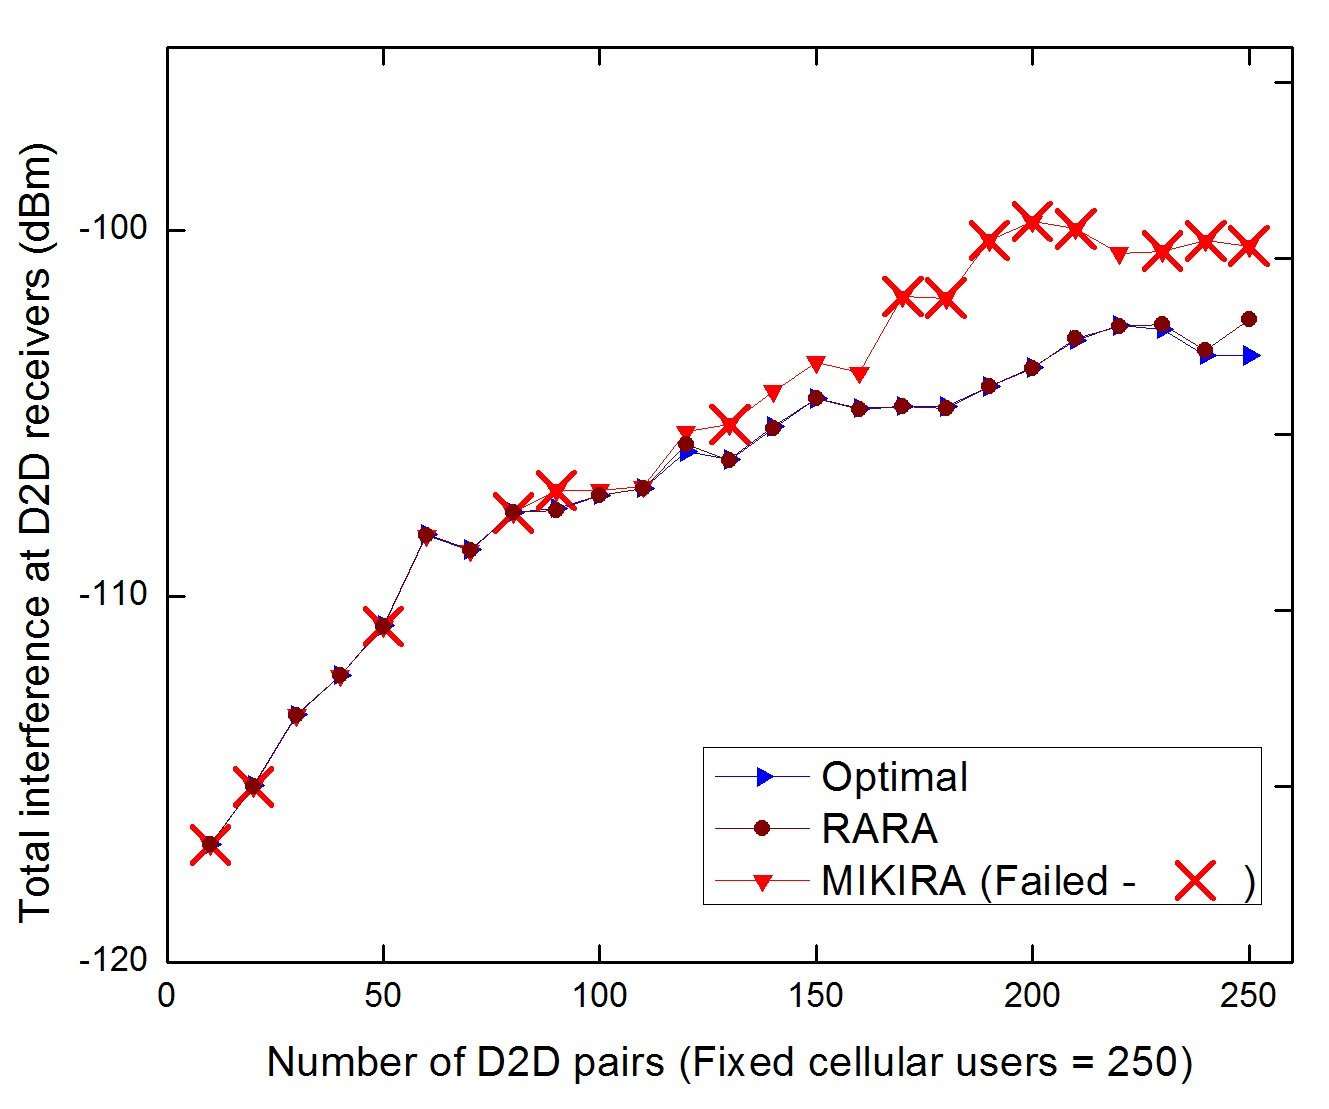
\includegraphics[width=\linewidth]{Graph/inter_d2d_rara.jpg}\par
	\caption{Comparison of total interference at the D2D receivers}
	\label{fig:inter_d2d_res}
	\end{subfigure}
	
	\hspace{12pt}
	\begin{subfigure}{.87\linewidth}
	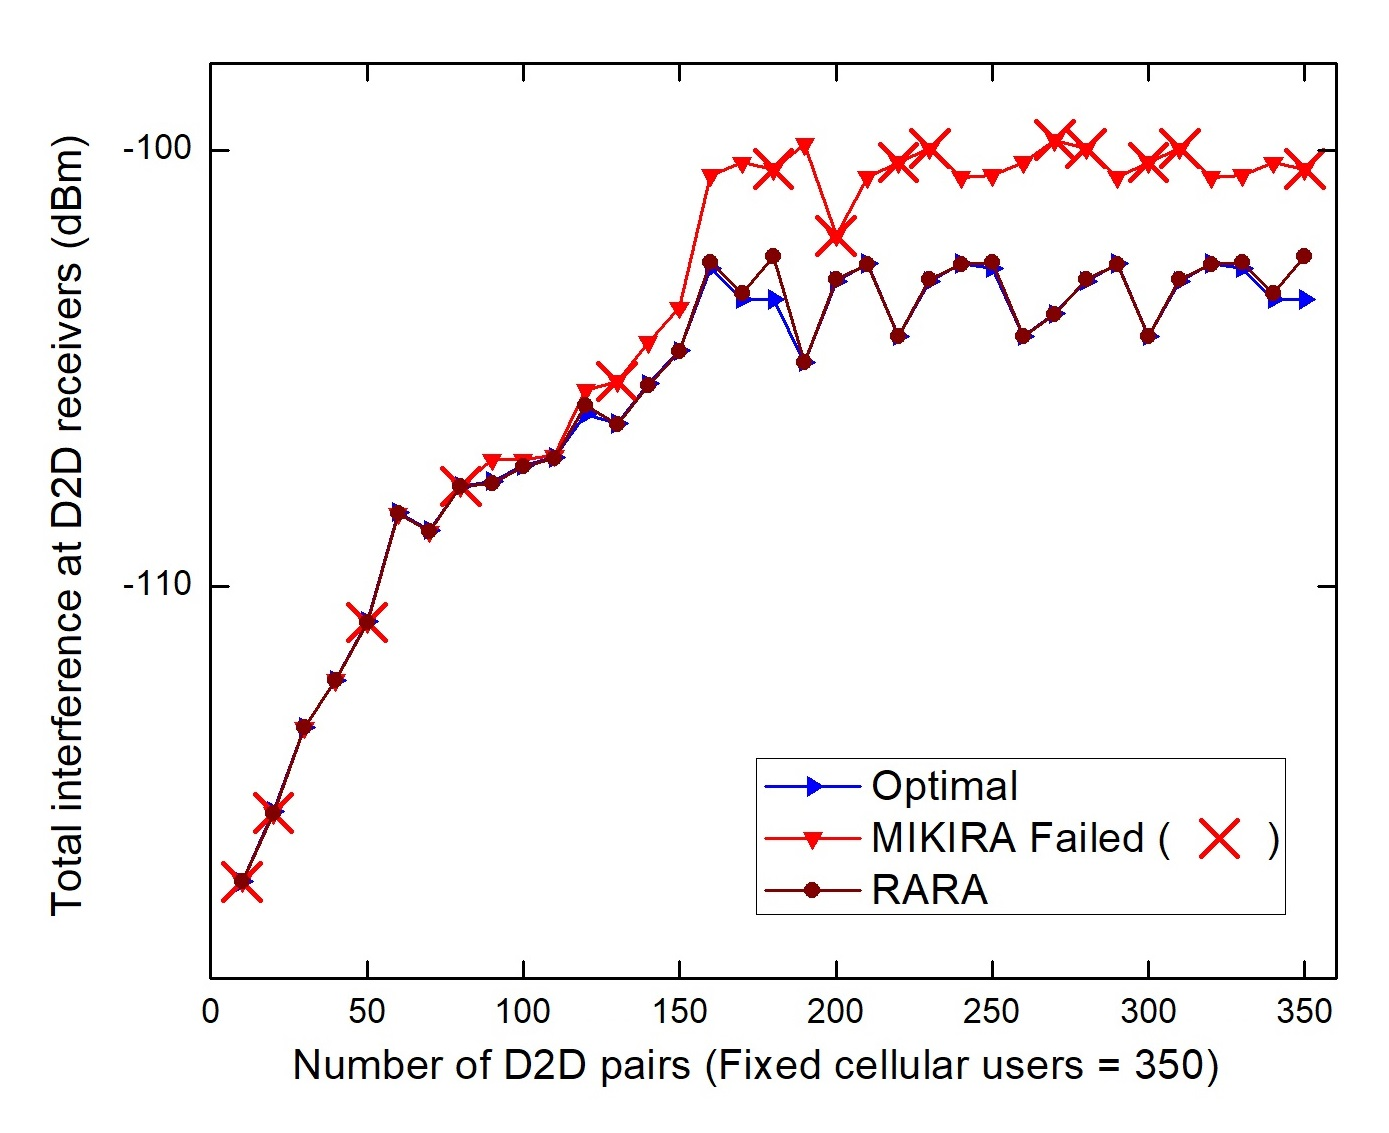
\includegraphics[width=\linewidth]{Graph/inter_d2d_rara_350.jpg}\par
	\caption{Comparison of total interference at the D2D receivers}
	\label{fig:inter_d2d_res_350}
	\end{subfigure}
	\end{multicols}
\caption{Performance comparisons among the resource allocation algorithms for restricted assignment}
\label{fig:res}
\end{figure*}


\smallskip
 
Though we prove that both TAFIRA and MIKIRA provide infeasible solutions in several cases which contradict the constraints (\ref{eqn:constraintxc}), (\ref{eqn:constraintFair}) and (\ref{eqn:constraintRestricted})  of the optimization problem, we present the comparison of the resource allocation algorithms for fair assignment in figure \ref{fig:fair} and for restricted assignment in figure \ref{fig:res}. As TAFIRA considers the fairness property of the problem, we compare the result of our fair assignment resource allocation (FARA) with the result of TAFIRA. Moreover, we compare the result of our restricted assignment resource allocation (RARA) with the result of MIKIRA as it does not guarantee the assignment of all D2D pairs.

\smallskip
 
Figure \ref{fig:inter_fair} and \ref{fig:inter_fair_350} represent the comparison of the total system interference due to sharing of RBs in case of fair assignment. Here, FARA algorithm produces less amount of interference than TAFIRA. We also find out the optimal solution of the problem (implementing integer linear program in ``Gurobi" \cite{gurobi}) and find that interference in FARA algorithm is  either optimal or very close to the optimal. Furthermore, in figure \ref{fig:inter_res} and \ref{fig:inter_res_350} shows the comparison of total system interference for restricted assignment. RARA algorithm produces less amount of interference than MIKIRA. Figure \ref{fig:inter_fair}, \ref{fig:inter_fair_350}, \ref{fig:inter_res} and \ref{fig:inter_res_350} also depict those cases where TAFIRA and MIKIRA fail (shown as $\times$ in the graphs) to produce feasible solutions even if such solutions exist. However, both FARA and RARA algorithm produces very close to optimal interference for their respective assignment types. Figure \ref{fig:inter_d2d_fair}, \ref{fig:inter_d2d_fair_350} and \ref{fig:inter_d2d_res}, \ref{fig:inter_d2d_res_350} represent the comparison of the total interference at D2D receivers for fair and restricted assignment respectively. Nonetheless, FARA and RARA algorithm introduce significantly less interference at D2D receivers than TAFIRA and MIKIRA. 


\begin{figure}[t]
\centering
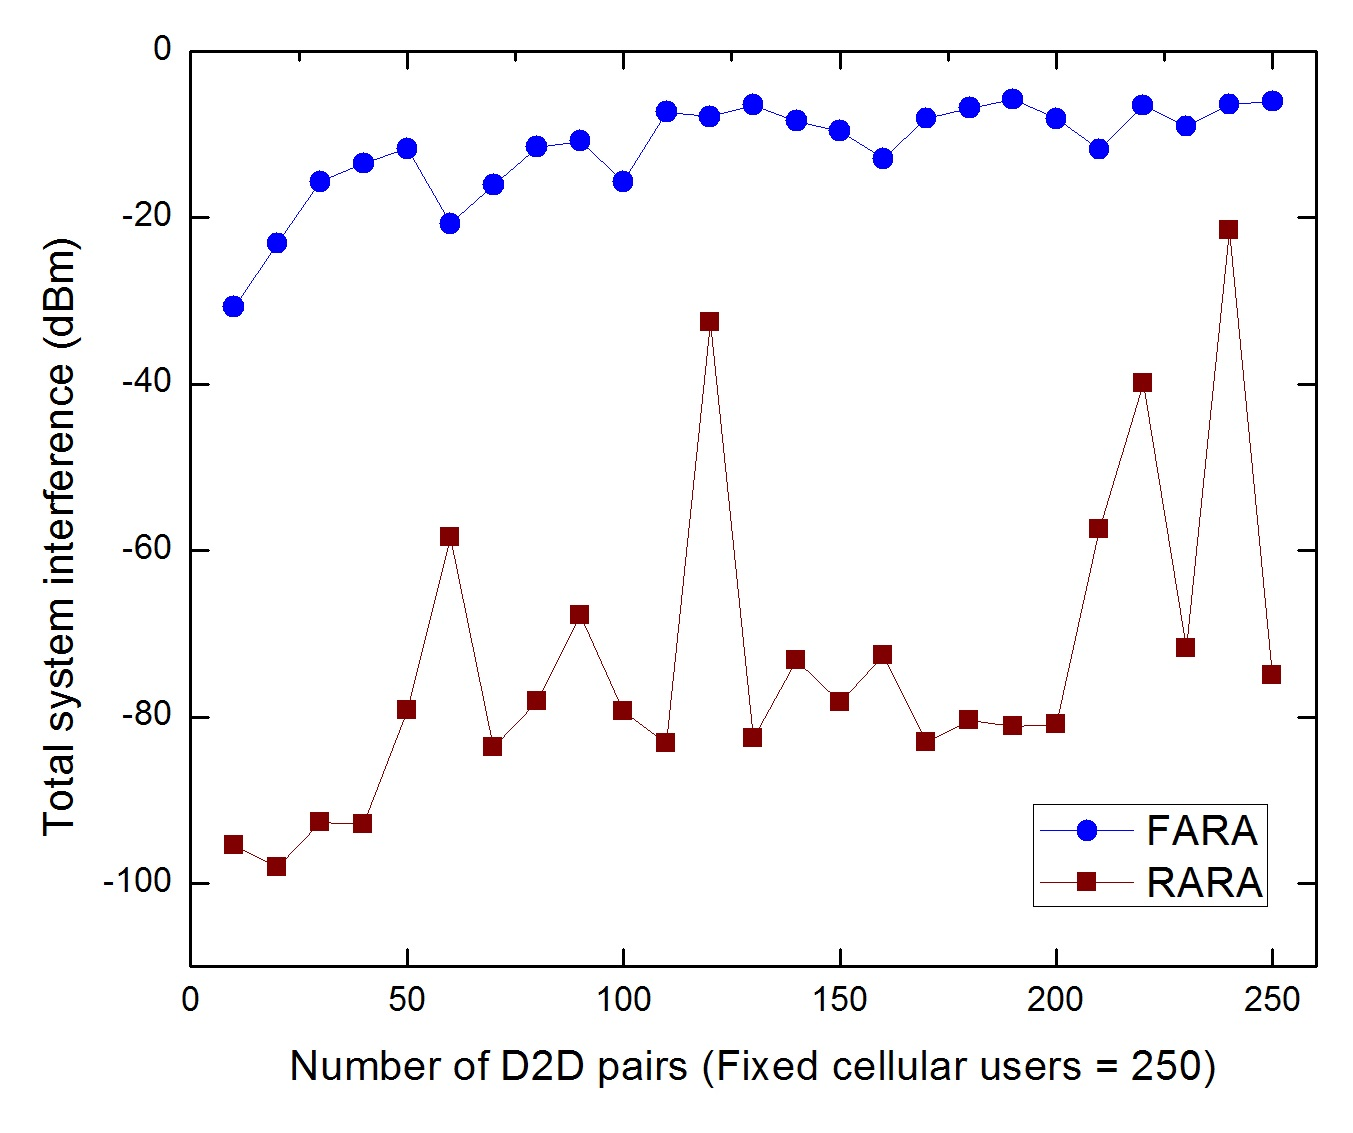
\includegraphics[width=85mm]{Graph/inter_rara_vs_fara.jpg}
\vspace{-0.3cm}
\caption{Comparison of Interference between FARA and RARA
\label{fig:fara_vs_rara)}}
\end{figure}


\smallskip
 
Figure \ref{fig:sumrate_fair}, \ref{fig:sumrate_fair_350} and \ref{fig:sumrate_res}, \ref{fig:sumrate_res_350} represent normalized system sum rate for fair and restricted assignment respectively. In both cases, all the results are normalized with respect to optimal system sum rate. Hence, optimal results in figure \ref{fig:sumrate_fair}, \ref{fig:sumrate_fair_350}, \ref{fig:sumrate_res} and \ref{fig:sumrate_res_350} is calculated using fair assignment and  restricted assignment respectively. It is clear that both RARA and FARA outperform TAFIRA and MIKIRA in terms of system sum rate. Moreover, TAFIRA and MIKIRA fail to achieve target sum rate in many cases, whereas FARA and RARA give the solution in those cases too. The difference in the system sum rate gets higher with the increased number of D2D pairs for the fixed number of cellular UEs. In the case of restricted assignment, some D2D pairs are not assigned with any cellular UEs as sharing RBs with those D2D pairs decrease the system sum rate as well as increase the system interference. Figure \ref{fig:fara_vs_rara)} shows that fair assignment produces more system interference than restricted assignment.

\smallskip
 
From various simulations, we also find that RARA algorithm assigns around 55\% to 65\% D2D pairs in average cases. From all the simulation graphs it is clear that, RARA algorithm gives lower system interference by sharing less D2D pairs where as FARA algorithm gives higher interference than RARA algorithm by giving a fair chance of sharing to all the D2D pairs and our proposed algorithm for both FARA and RARA outperforms TAFIRA and MIKIRA in all the cases.

\smallskip
 
It can be noticed that the curves of the simulation graphs are neither smooth nor monotonic but consistent. As the locations of the D2D pairs and cellular UEs are generated randomly in each run, the results are not monotonic. Furthermore, some random cases are generated where the results change very much (from high to low and vice versa), generating spikes in the curves in both upward and downward direction. This graphs also prove that multiple scenarios are accumulated in one place, which saves us from number of graphs for each scenario. 
 
\smallskip
 
In summary, our proposed algorithm returns the assignment which introduces interference very close to the optimal interference by satisfying the sum rate demand in both of the approaches (FARA and RARA). In addition, our proposed algorithm returns better system sum rate than TAFIRA and MIKIRA while introducing less amount of total system interference. Unlike TAFIRA and MIKIRA, our algorithm guarantees a solution provided that such solution exists and also introduces less interference than TAFIRA and MIKIRA at D2D receivers. 

\section{Conclusion}\label{sec:conclusion}
\smallskip
 
Interference minimization in D2D communication underlaying cellular network is addressed in this paper. We propose two phase resource allocation algorithms for two types of assignment in D2D communication. One is the fair assignment where all D2D pairs have the flexibility to share RBs of exactly one cellular UEs and another one is the restricted assignment where D2D pairs are blocked to share RBs of any cellular UEs if their sharing decreases the sum rate. In phase-I, we formulate the problem as a weighted bipartite matching problem and use the Hungarian algorithm to minimize the interference and get a feasible initial solution. In some cases, phase-I of the proposed algorithm may not provide the lowest possible interference. Phase-II of our proposed algorithm is based on local search technique that starts with feasible solutions given by the corresponding phase-I of the proposed algorithm and tries to minimize the total system interference. We find that our proposed algorithm always guarantees solutions whenever they exist. Simulation results suggest that in the all the cases, our proposed algorithm returns either optimal or very close to the optimal solutions and outperforms existing algorithms. Although sharing RBs of a single cellular UE with more than one D2D pair generates higher interference and sharing RBs of different cellular UEs by a single D2D pair makes the system complex, proper resource allocation algorithm can mitigate the problem. We plan to investigate this issue in our future work.
 

\section*{Acknowledgment}
\smallskip

Authors of this paper are extremely grateful to the anonymous reviewers for their rigorous criticism about this work which help the authors to shape out this research work in excellence.





\bibliographystyle{IEEEtran}
\bibliography{bibfile}
\vspace{-50pt}
\begin{IEEEbiography}[{
\includegraphics[width=1in,height=1.25in,clip,keepaspectratio]{yeakub.jpg}}]{\textbf{Md. Yeakub Hassan}} received the B.Sc. degree in computer science and engineering from the Islamic University of Technology, Bangladesh, in 2016. He is currently serving the Department of Computer Science and Engineering, Green University of Bangladesh, as a Lecturer. Formerly he was an assistant database engineer in computer center of Islamic University of Technology. His research interests include Internet of Things, Data structures and Algorithms, Cellular Automata, Systems and Networking, Optimization and Graph Theory.
\end{IEEEbiography}

\vspace{-45pt}
\begin{IEEEbiography}[{
\includegraphics[width=1in,height=1.25in,clip,keepaspectratio]{faisal.jpg}}]{\textbf{Faisal Hussain}}  received the B.Sc. degree in computer science and engineering from the Islamic University of Technology, Bangladesh, in 2016. He is currently serving the Computer Centre of Islamic University of Technology, as an Assistant Programmer. His research interests include internet of things, computer networks, wireless communication and network security.
\end{IEEEbiography}

\vspace{-45pt}
\begin{IEEEbiography}[{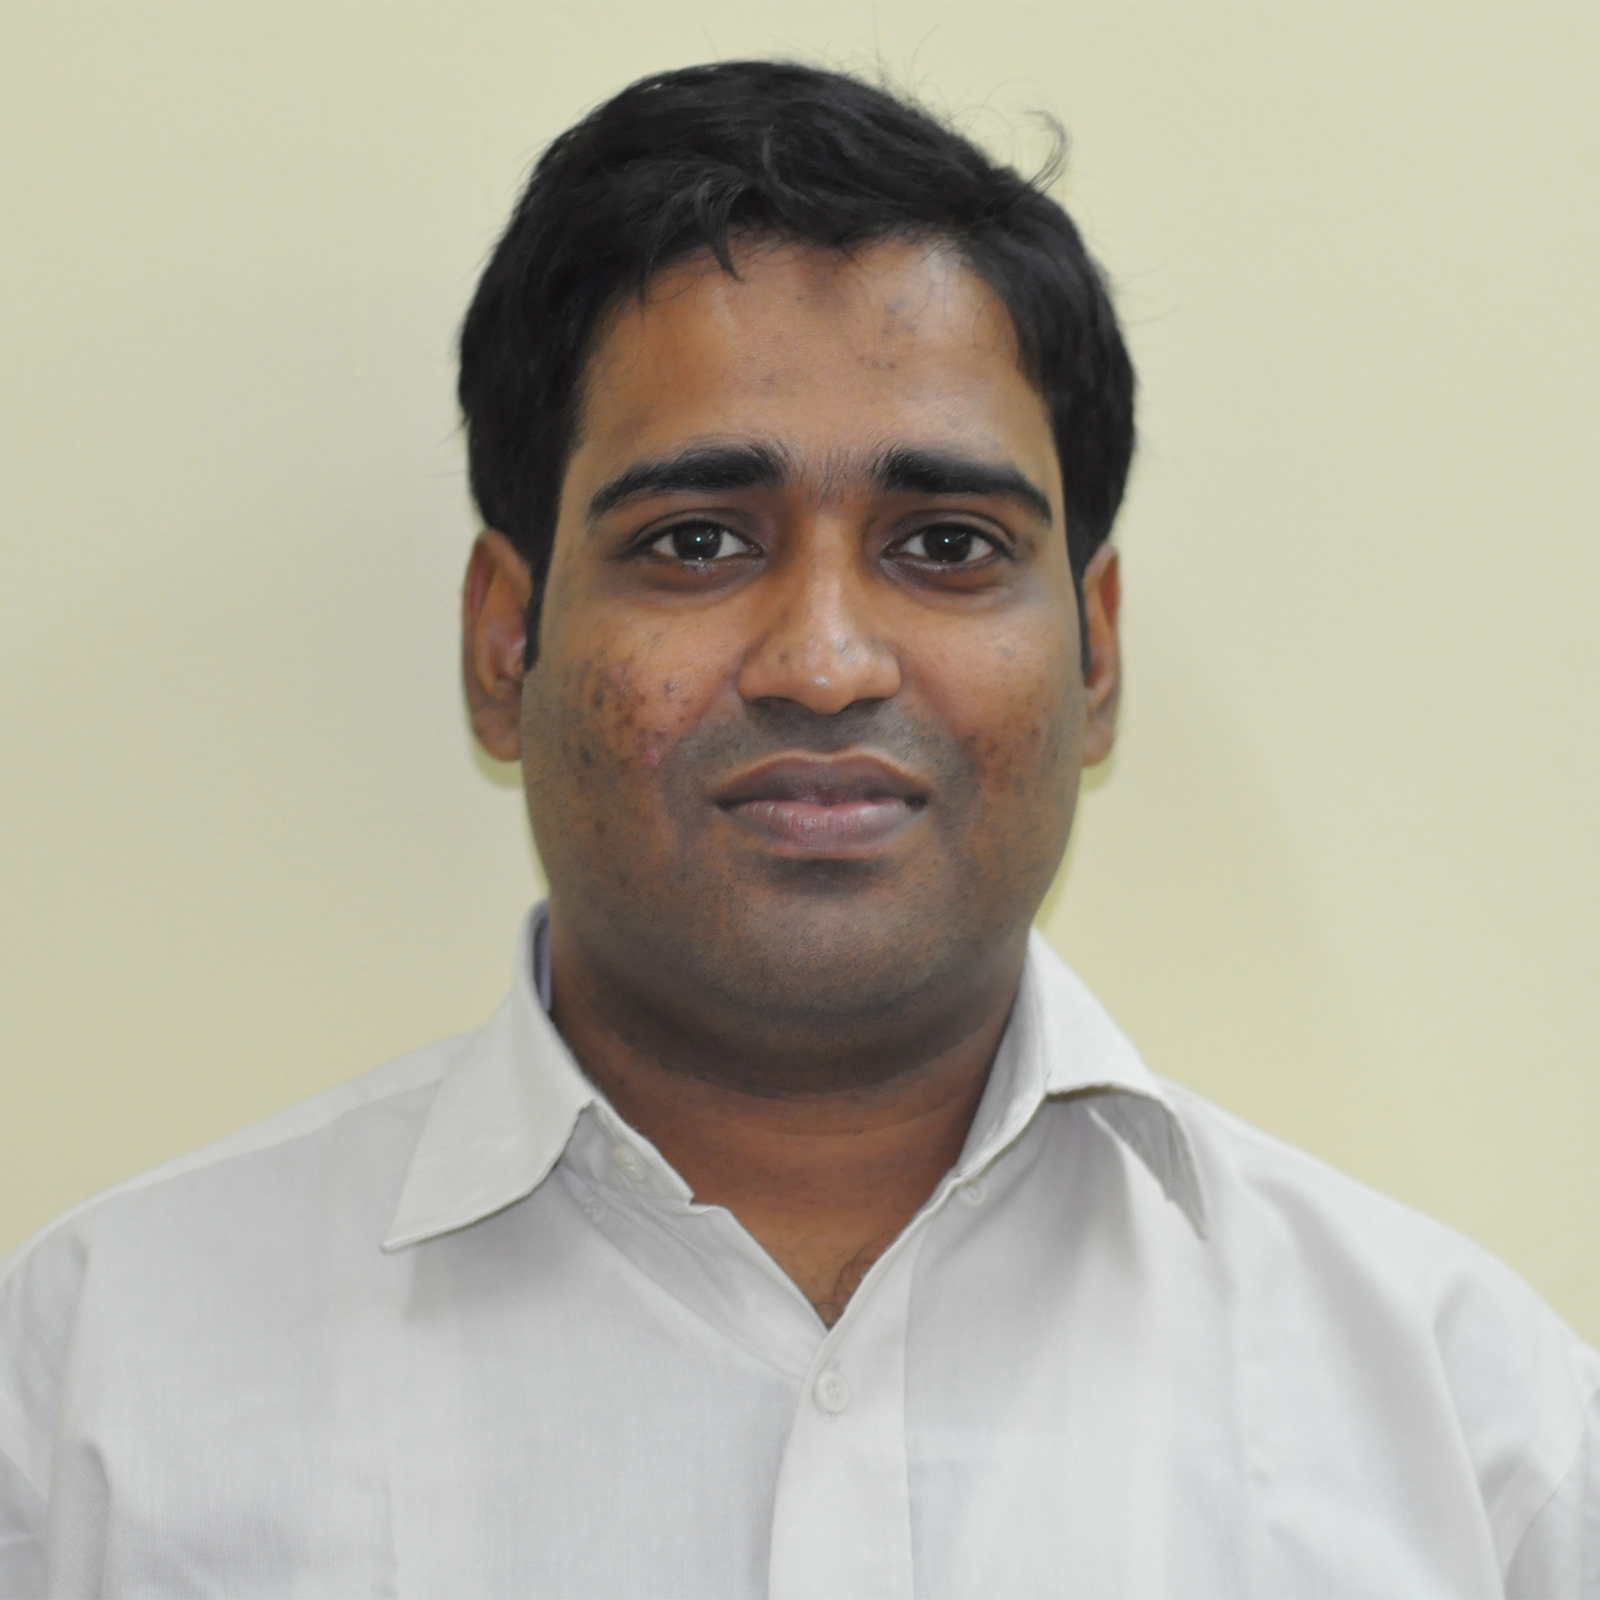
\includegraphics[width=1in,height=1.25in,clip,keepaspectratio]{saki.jpg}}]{\textbf{Md. Sakhawat Hossen}}  is doing his PhD in the department of Computer Science and Engineering (CSE) of the Islamic University of Technology (IUT), Gazipur, Bangladesh. He has completed his MSc in Internetworking from the Royal Institute of Technology (KTH), Sweden. He received his BSc degree in Computer Science and Information Technology from Islamic University of Technology (IUT), Gazipur, Bangladesh. Currently he is also serving the CSE department of the Islamic University of Technology (IUT) as an assistant professor. Formerly he was a lecturer in the department of CSE of Stamford University Bangladesh and
he also served the CSE department of American International University Bangladesh (AIUB) as an assistant professor. His research interest is mainly focused on D2D communication, RFID, Cellular Automata, Combinatorial and evolutionary optimization problems, Internet security, wireless sensor network (WSN), IP network and VoIP.
\end{IEEEbiography}

\vspace{-45pt}
\begin{IEEEbiography}[{
\includegraphics[width=1in,height=1.25in,clip,keepaspectratio]{salimur.jpg}}]{\textbf{Salimur Choudhury}}  is an assistant professor in the department of Computer Science at
Lakehead University, ON, Canada. He received PhD in Computing from Queen's University,
ON, Canada in 2012. His research interests include designing algorithms for wireless
communication, optimization, cellular automata, approximation algorithms, etc.
\end{IEEEbiography}

\begin{IEEEbiography}[{\includegraphics[width=1in,height=1.25in,clip,keepaspectratio]{mma.jpg}}]{\textbf{Muhammad Mahbub Alam}}  received his B.S. degree in Applied Physics and Electronics and
M.S. degree in Computer Science from the University of Dhaka, Bangladesh in 1998 and 2000,
respectively. He received his Ph.D. from Kyung Hee University, South Korea in February
2009. Currently he is working as a professor and the head of the department of Computer
Science and Engineering (CSE) of the Islamic University of Technology (IUT), Gazipur,
Bangladesh. He has worked as a Research Faculty in Kyung-Hee University until April, 2010.
Since 2002, he has been working as a faculty member in the Computer Science and
Information Technology (CIT) department in Islamic University of Technology (IUT), Dhaka,
Bangladesh. His research interests include wireless networking and performance modeling
and analysis of networking systems, optimization problems, wireless sensor network (WSN),
and Internet of Things (IoT).
\end{IEEEbiography}



\EOD

\end{document}
